%% bare_conf.tex
%% V1.4b
%% 2015/08/26
%% by Michael Shell
%% See:
%% http://www.michaelshell.org/
%% for current contact information.
%%
%% This is a skeleton file demonstrating the use of IEEEtran.cls
%% (requires IEEEtran.cls version 1.8b or later) with an IEEE
%% conference paper.
%%
%% Support sites:
%% http://www.michaelshell.org/tex/ieeetran/
%% http://www.ctan.org/pkg/ieeetran
%% and
%% http://www.ieee.org/

%%*************************************************************************
%% Legal Notice:
%% This code is offered as-is without any warranty either expressed or
%% implied; without even the implied warranty of MERCHANTABILITY or
%% FITNESS FOR A PARTICULAR PURPOSE!
%% User assumes all risk.
%% In no event shall the IEEE or any contributor to this code be liable for
%% any damages or losses, including, but not limited to, incidental,
%% consequential, or any other damages, resulting from the use or misuse
%% of any information contained here.
%%
%% All comments are the opinions of their respective authors and are not
%% necessarily endorsed by the IEEE.
%%
%% This work is distributed under the LaTeX Project Public License (LPPL)
%% ( http://www.latex-project.org/ ) version 1.3, and may be freely used,
%% distributed and modified. A copy of the LPPL, version 1.3, is included
%% in the base LaTeX documentation of all distributions of LaTeX released
%% 2003/12/01 or later.
%% Retain all contribution notices and credits.
%% ** Modified files should be clearly indicated as such, including  **
%% ** renaming them and changing author support contact information. **
%%*************************************************************************


% *** Authors should verify (and, if needed, correct) their LaTeX system  ***
% *** with the testflow diagnostic prior to trusting their LaTeX platform ***
% *** with production work. The IEEE's font choices and paper sizes can   ***
% *** trigger bugs that do not appear when using other class files.       ***                          ***
% The testflow support page is at:
% http://www.michaelshell.org/tex/testflow/


\documentclass[conference]{IEEEtran}
\usepackage{subfigure}
\usepackage{xcolor}
\usepackage{url}
\usepackage{mathrsfs}
\usepackage{amsfonts}
\usepackage[normalem]{ulem}
\usepackage{array}
\usepackage{amsmath}
%\usepackage{underscore}
\usepackage{graphics}
\usepackage{graphicx}
\usepackage{algorithm}
\usepackage{algorithmic}
\usepackage{caption}
\newcommand{\argmin}{\arg\!\min}
\newcommand{\argmax}{\arg\!\max}


\usepackage[utf8]{inputenc}
\usepackage[english]{babel}
\newtheorem{theorem}{Theorem}[section]
\newtheorem{corollary}{Corollary}[theorem]
\newtheorem{lemma}[theorem]{Lemma}



% *** GRAPHICS RELATED PACKAGES ***
%
\ifCLASSINFOpdf
  % \usepackage[pdftex]{graphicx}
  % declare the path(s) where your graphic files are
  % \graphicspath{{../pdf/}{../jpeg/}}
  % and their extensions so you won't have to specify these with
  % every instance of \includegraphics
  % \DeclareGraphicsExtensions{.pdf,.jpeg,.png}
\else
  % or other class option (dvipsone, dvipdf, if not using dvips). graphicx
  % will default to the driver specified in the system graphics.cfg if no
  % driver is specified.
  % \usepackage[dvips]{graphicx}
  % declare the path(s) where your graphic files are
  % \graphicspath{{../eps/}}
  % and their extensions so you won't have to specify these with
  % every instance of \includegraphics
  % \DeclareGraphicsExtensions{.eps}
\fi


% correct bad hyphenation here
\hyphenation{op-tical net-works semi-conduc-tor}


\begin{document}
%
% paper title
% Titles are generally capitalized except for words such as a, an, and, as,
% at, but, by, for, in, nor, of, on, or, the, to and up, which are usually
% not capitalized unless they are the first or last word of the title.
% Linebreaks \\ can be used within to get better formatting as desired.
% Do not put math or special symbols in the title.
\title{``The Lull before the Storm": Event Detection\\ from Group Anomaly}

%\title{Group Anomaly Detection using Graph Wavelet}
% author names and affiliations
% use a multiple column layout for up to three different
% affiliations

%\author{Fang Jin\footnotemark[1], Feng Chen\footnotemark[2], Rupinder Paul Khandpur\footnotemark[1], Chang-Tien Lu\footnotemark[1], Naren Ramakrishnan\footnotemark[1]\\[2mm]
%		\affaddr\footnotemark[1] {Discovery Analytics Center, Department of Computer Science, Virginia Tech.}\\
%\affaddr\footnotemark[2] {Department of Computer Science, University at Albany, SUNY}\\[0.5mm]
%        \footnotemark[1] \email {\{jfang8, rupen, ctlu, naren\}@cs.vt.edu }, \footnotemark[2] \email {fchen5@albany.edu}
%}
%\author{\IEEEauthorblockN{Fang Jin}
%\IEEEauthorblockA{Discovery Analytics Center\\
%Department of Computer Science\\
%Virginia Tech\\
%Email: jfang8@cs.vt.edu}
%\and
%\IEEEauthorblockN{Feng Chen and \\ Rupinder Paul Khandpur}
%\IEEEauthorblockA{Department of Computer Science\\
%University at Albany, SUNY\\
%Virginia Tech\\
%Email: fchen5@albany.edu, rupen@cs.vt.edu}
%\and
%\IEEEauthorblockN{Chang-Tien Lu and\\ Naren Ramakrishnanu}
%\IEEEauthorblockA{Discovery Analytics Center\\
%Department of Computer Science\\
%Virginia Tech\\
%Email: ctlu@vt.edu, naren@cs.vt.edu}
%}



% make the title area
\maketitle

% As a general rule, do not put math, special symbols or citations
% in the abstract
\begin{abstract}
Event detection in online social media has primarily focused on identifying
abnormal spikes, or bursts, in activity. However, disruptive events such as socio-economic disasters, civil unrest, and even power outages, often result in abnormal troughs involving group absenteeism of activity. We present the first study, to our knowledge, that models absenteeism and uses detected absenteeism as a basis for event detection in location based social networks (LBSN) such as Twitter. Our framework addresses the challenges of (i) early detection of absenteeism, (ii) identifying the point of origin, and (iii) identifying groups or communities underlying the absenteeism. Our approach uses the formalism of graph wavelets to represent the spatiotemporal structure and user activity in a LSBN. This formalism affords multiscale analysis, enabling us to detect anomalous behavior at different graph resolutions, which in turn allows identification of event location and anomalous groups underlying the network. We introduce a systematic group anomaly detection method using graph wavelets to detect absenteeism group and burst group simultaneously.
The effectiveness of our approach is verified with protest events involving Twitter activity over Latin American countries.
\end{abstract}

% no keywords
% For peer review papers, you can put extra information on the cover
% page as needed:
% \ifCLASSOPTIONpeerreview
% \begin{center} \bfseries EDICS Category: 3-BBND \end{center}
% \fi
%
% For peerreview papers, this IEEEtran command inserts a page break and
% creates the second title. It will be ignored for other modes.
\IEEEpeerreviewmaketitle


\section{Introduction}
\label{sec:introduction}
Social Microblogs such as Twitter and Weibo are experiencing explosive growth, with billions of users globally sharing their daily status updates online.
For example, Twitter has more than 310 million average monthly active users (78\% from mobile) as of March 31, 2016, and an estimated increase of 25\% per year\footnote{http://www.statista.com/statistics/282087/number-of-monthly-active-twitter-users/}.
Various studies have shown that Twitter is viable as a social ``sensor'', and holds great promise for detecting and forecasting significant societal events~\cite{bugel2013multilingual,sakaki2010earthquake}.
In recent years, a significant body of research~\cite{aggarwal2012event,hong2012discovering,lappas2009burstiness,lappas2012spatiotemporal,sakaki2010earthquake,sayyadi2009event,watanabe2011jasmine,weng2011event,yin2011geographical} has focused on modeling bursts and increases of user activity in social media.

However, real world events are not only correlated with burst signals, but can also exhibit unusually low levels of activity in social networks.
As shown in Figure 1, a protest in the city of Natal, Brazil began at 5:00 PM (local time) at the Museum of the Republic, with people gradually joining the demonstration. %\footnote{http://www.jb.com.br/pais/noticias/2013/06/17/manifestantes-invadem-cobertura-do-congresso-nacional-em-brasilia/}.
On Twitter, there was an uncharacteristic lull in activity or {\it group absenteeism} behavior from 6:00 PM---8:00 PM on the same day.
Another example comes from December 24, 2013, southern Brazil experienced widespread flash floods. According to news sources, more than 50,000 people were forced to flee their homes in Minas Gerais and Espirito Santo, in the southern states of Brazil. Immediately following the floods, Twitter activity in this region dropped by 51\%, and reached its lowest point that evening.
%Other examples of \textit{group absenteeism} that we observed from Latin American Twitter activity include bus strikes in Brazil on May 21, 2014, the Iquique earthquake in Chile on April 1, 2014, and a major power supply disruption in Argentina on December 30, 2013.

\begin{figure}[t]
\centering
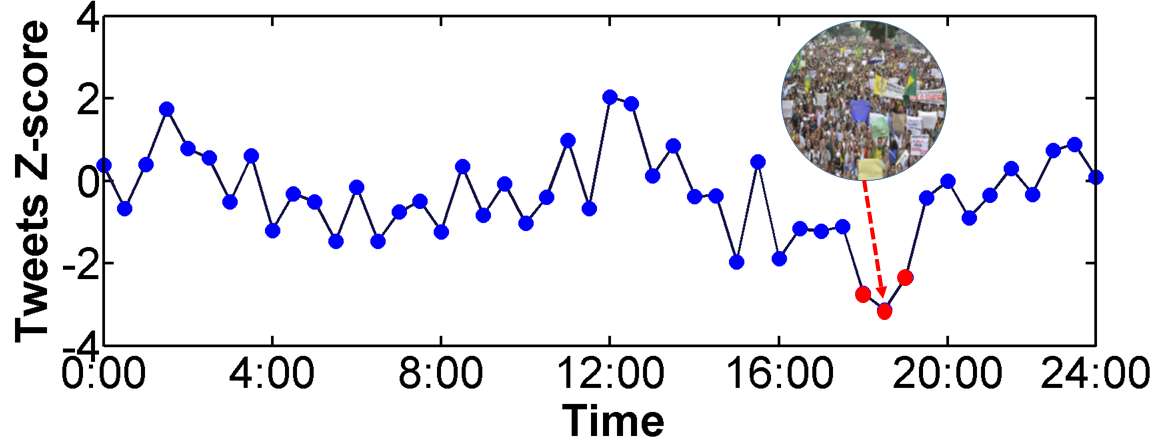
\includegraphics[height=1.1in]{figures/Natal_example1.png}
\caption{Detected group absenteeism in Natal, Brazil beginning at 6:00 PM on June 17, 2013. This absenteeism event coincides with a large protest that happened in the region.}
\label{fig:natal-protest}
\end{figure}
Investigating this phenomenon of unusually calm behavior online holds enormous potential for understanding localized, disruptive societal events.
In this paper we focus on group anomaly detection which is not only able to capture burst events, but also absenteeism events, and introduce this important topic as a key data mining task for social media analytics.
An \textit{absenteeism} event in social networks can be defined as an event which is characterized by a significant lull in activity such as a sudden, sharp decrease of Twitter volume within a short period of time (and which may precedes a major burst in re-activity).
This paper presents the first study to systematically investigate group anomaly in Location Based Social Networks.
To appropriately incorporate absenteeism concepts into our detection approach, we must first address the following questions
\begin{itemize}
\item How to define group anomaly in graph? How to reconcile both burst and absenteeism scenarios?
\item What scale should we select to model the abnormal groups? Which node should be the central point?
\item What is the most efficient approach to select abnormal groups that are spatially and temporally localized?
\item How do we model an absenteeism signal for event detection? Even though we have clear examples of real world events which can explain the observed absenteeism, not all absenteeism occurrences can be associated with underlying events. Therefore we must be able to differentiate absenteeism from noisy signals for event detection.
\end{itemize}

Graph wavelet approach display several outstanding advantages to study the above
questions: scalability, localization, low computational complexity, and group compact. In this scenario, the data objects are embedded in a general graph as vertices.
By employing wavelet transforms on the graph, we can construct a wavelet function with a graph structure. We propose the graph anomaly index depends on graph structure and absenteeism score vector, which can define whether a graph is abnormal. When the graph is abnormal, we will calculate its wavelet coefficient, to identify the central node and its coverage cities. In this way, we are able to select abnormal groups at different scales. The group anomaly detection methods are varied and proved to be effective in events detection such as man-made protest and natural disasters.

%As for another abnormal scenarios such as natural disaster, we propose a two-pass group anomaly detection method that first detects absenteeism, and then checks if there is a subsequent burst in activity within a specific time period. By comparing correlations between the wavelet coefficients of both of these groups, we are able to capture a possible real world event.

Our contributions are thus:
\begin{itemize}
\item To the best of our knowledge this is the first study to modeling group absenteeism as a basis for event detection. We study different group anomaly, either burst or absenteeism, and prove those anomaly is indicative at detecting events such as man-made protests or natural disasters.
\item We incorporate graph wavelets as a mechanism to detect the most anomalous subgraphs at different scales. We demonstrate how this is a powerful approach for social media analytics.
\item We define the graph anomaly index, which can decide whether a graph is abnormal. Furthermore, we are able to locate the central node and identify the abnormal groups.
%\item We propose a novel two-pass event detection method that uses correlation scores between the group depicting \textit{absenteeism} and the group demonstrating increased activity to probabilistically determine the likelihood of an event.
\end{itemize}

The rest of the paper is organized as follows. Section~\ref{sec:related} reviews related work and existing methodologies and Section~\ref{sec:problem} formalizes the research problem. In Section~\ref{sec:algorithm}, we discuss the graph wavelet formalism for group anomaly detection.
%and subsequently demonstrate how it can be used for two-pass event detection.
Section~\ref{sec:experiment} presents extensive experiments for event detection, and the paper concludes with a summary of the research in Section~\ref{sec:conclusion}.


\section{RELATED WORK}
\label{sec:related}
\paragraph{Group Anomaly Detection}
Anomaly detection in Graphs has been well studied using outlier detection~\cite{akoglu2009anomaly}. When considering group concept, two directions has been studied~\cite{akoglu2015graph}: one is anomalies in unlabeled/plain graphs~\cite{noble2003graph}, the other is in attributed graphs. In the plain graph anomaly detection, since the only given information is its structure, various features such as distances, communities~\cite{sun2005neighborhood} have been employed to define graph anomaly. In work of~\cite{henderson2010metric}, more metrics like vertices, edges, degree, weight, connected components are incorporated into detection framework. In attributed graphs, features regarding nodes behaviors make it possible to have a richer graph representation, which is usually tied with some real-world applications. Such as \cite{yu2014glad} defines the group based on the term of role, and model the normal groups follow the same pattern with respect to their role mixture rates. Other approaches to group anomaly detection include building generative models of group anomalies~\cite{xiong2011hierarchical} where the goal is to automatically infer the groups and detect group anomalies in a social network. Typical to mixture models such methods suffer from high computational complexity due to the size of data and are heavily parameterized. In our work, we consider both graph structure and nodes features, propose a graph wavelet based approach for group anomaly detection, which can guarantee the detected group to be automatically compact, with linear computation complexity and scalability.

\paragraph{Event Detection}
Event detection based on LSBNs is a research area that has attracted significant attention in the last years. Traditional approaches focus on capturing spatiotemporal burstiness of keywords~\cite{lappas2009burstiness,lappas2012spatiotemporal}, Kalman filtering to track the geographical trajectories of hot spots of Tweets related to earthquakes~\cite{sakaki2010earthquake}; detecting topics of interest that are coherent in geographic regions~\cite{eisenstein2010latent,hong2012discovering,yin2011geographical}; applying clustering-based approaches search for emerging clusters of documents or terms using predefined similarity metrics that consider factors such as term co-occurrences and social interactions~\cite{aggarwal2012event,sayyadi2009event,watanabe2011jasmine,weng2011event}; and using the notion of compactness of a graph~\cite{rozenshtein2014event} to detect events. Several statistical methods have also been used, based on Kulldroff's spatial scan statistic\cite{kulldorff1997spatial}, to detect spatial outliers~\cite{chen2008detecting} and have been applied to a wide variety of domains including transportation networks, civil unrest forecasting~\cite{zhao2014unsupervised}, and heterogeneous social media graphs~\cite{chen2014non}.

Our approach to event detection problem is conceptually different from above mentioned studies. It includes a graph-theoretic framework to detect group anomaly and correlate them with future events. Although group absence behavior has been widely studied in the area of organizational behavioral studies~\cite{gaudine2001effects,seamonds1982stress}, it remains unexplored in the area of social network analysis. Resembling closely to group anomaly detection in complex networks, our detection approach is further distinguished by its focus on groups rather than individuals.

\paragraph{Graph Wavelet}
One of key challenges of our research problem is adapting the detection procedure for both missing and bursty activity groups. For this purpose, we incorporate spectral graph wavelets~\cite{hammond2011wavelets} into our algorithm. This strategy has been quite effectively used in multiscale community mining~\cite{tremblay2014graph}.
Wavelet methods based on spectral graph theory have been applied in a wide array data mining areas such as community detection, anomaly detection~\cite{calderara2011detecting} and other machine learning tasks~\cite{shuman_ACHA_2013,ghosh2003wavelet,rustamov2013wavelets,2000wavecluster}. By constructing wavelets over graphs we are able take advantage of local information encoded in graph structure and then cluster and identify nodes which are similar in a scale-dependent fashion.

\section{PROBLEM SETTING}
\label{sec:problem}
In this section, we first introduce mathematical notations. Then we formalize our approach to group anomaly detection.
We first describe the accompanying notations in section~\ref{sec:notations} which will be used throughout the paper.
Then we formally present problem statement, provide a brief comparison of our approach to conventional solutions, and review the challenging issues that are relevant to event detection problem.
\subsection{Notations}
\label{sec:notations}
Given an undirected, weighted graph $\mathbf{G}(V,E;f)$, where $V=\{v_0,v_1,...,v_{N-1}\}$ represents the set of $N$ cities, $E$ refers to the connections between neighboring cities. $W$ is a matrix of non-negative weights associated with each edge, where $e_{ij}\in E$. The function, $f: V \rightarrow {\mathbb{R}}^N$ maps the vertices of graph $\mathbf{G}$, and $f(n)$ stands for the value on the vertex $v_n$. Graph $\mathbf{G}$'s adjacency matrix $\mathbf{A}$ is of size $N\times N$, where each element $a_{ij}$ is represented as:
\begin{equation}
a_{ij} = \left\{ \begin{array}{rl}
 w_{ij} &\mbox{ when $e_{ij}\in {E}$} \\
  0 &\mbox{ otherwise}
       \end{array} \right.
\end{equation}
Here, $\mathbf{A}$ is symmetric since $a_{ij}=a_{ji}$.
Let $d_i=\sum\limits_{v_j \in V}a_{ij}$ be the sum of all edge weights that are incident on $v_i$, and $\mathbf{D}$ be the diagonal matrix denoted as $\mathbf{D}=diag\{d_1,d_2,\ldots,d_N\}$. A Laplacian matrix $\mathcal{L}$ is defined as $\mathcal{L}=\mathbf{D-A}$. It is a symmetric matrix and has real eigenvalues $\lambda_{i}$ such that $0 = \lambda_{0} < \lambda_{1} \leq \lambda_{2} \leq \ldots \leq \lambda_{N-1} = \lambda_{max}$. The complete set of $\mathcal{L}$'s normalized eigenvectors~\cite{bapat2010graphs} $\chi_{i}$ for $i=0,1,2,...,N-1$ is described as:
\begin{equation}
\label{eq:eigenvalues}
\mathcal{L}\chi_{i}=\lambda_{i}\chi_{i}
\end{equation}
The set of eigenvalue and normalized eigenvector pair is denoted as:
\begin{equation}
\label{eq:spectrum}
\sigma({\mathbf{G}}):=\{(\lambda_l,\chi_l)\}_{l=0}^{N-1}.
\end{equation}$\sigma({\mathbf{G}})$ is also called graph spectrum of $\mathbf{G}$.




\subsection{Problem Statement}
\label{sec:problemformulation}
We focus on the problem of group anomaly detection from online social networks, based on the absenteeism behavior observed in user activity in geographically proximal communities or group of cities.
Conventionally, this problem can be described as following: \emph{given a graph and \textit{absenteeism score} vector, $\mathbf{G}(V,E;f^t)$ at time interval $t$, select a subset $\Sigma \subseteq V$, such that
\begin{eqnarray}
 \label{eq: problem}
    \Sigma=\underset{P\subseteq V, P \mbox{ is compact}}{\arg\min}\ \ \sum_{v_k\in P} {f(k)}
\end{eqnarray} }
However, how to define compactness of the selected subset $\Sigma$ is an open problem.
A general solution to this problem is employing a combinatorial optimization method, by defining a constrained objective function over a network one can identify a subset of vertices which maximize the corresponding function~\cite{rozenshtein2014event}. Therefore, Equation~\ref{eq: problem} can be modified as:
\begin{eqnarray}
 \label{eq: problem_conventional}
    \Sigma=\underset{P\subseteq V}{\arg\min}\ \ \sum_{v_k\in P} {f(k)}+\lambda \mu(P)
\end{eqnarray}
, where $\mu(P)$ is the compactness penalty function of $P$ (e.g., the sum of distances among
all pairs of the vertices in $P$~\cite{rozenshtein2014event}), and $\lambda$ is the regularization parameter.
However, such methods suffer from the following issues:
\begin{enumerate}
\item Definition of the compactness function $\mu(P)$ is subjective.
%To define and measure the compactness of subset $P\subseteq V$ is challenging, considering the exponential varieties of complex graphs.
\item  Determination of an appropriate regularizer $\lambda$ is difficult, as we do not have sufficient training data for this purpose.
%To determine a suitable regularization parameter $\lambda$ in the objective function is ambiguous, because simply combining multiple physical different concepts in the objective function makes the optima sensitive to $\lambda$.
\item To solve this objective function is often a NP-hard problem, which makes it unpractical in many real world applications. Sometimes, even the approximate solutions are of high computation complexity, if there are any.
\end{enumerate}
In contrast, we proposed a novel group anomaly detection algorithm in social networks using spectral graph wavelet theory.
The graph wavelets focus on the intrinsic geometric structure of the graph by transforming each vertex $v_i\in V$, and mining the topological information of both local and global centered vertices to support multiscale analysis.
In addition, the graph wavelet approach identifies abnormal groups which are automatically compact, and provides a fair and low computational method in terms of complexity for identifying abnormal group behavior in a broad application scenarios.


\section{ALGORITHMS}
\label{sec:algorithm}

In this section, we first introduce Graph Fourier Transform concept, explain eigenvector and eigenvalue meanings, then based on that define anomaly index of graph. The next is to describe graph wavelet's features such as reconstruction and localization. In section~\ref{sec:Group_Anomaly_Detection_via_graph_wavelet}, we propose the group anomaly detection algorithm via graph wavelet.
%And in section~\ref{sec:Group Absenteeism Event Detection} we present the two-pass event detection algorithm.

\subsection{Graph Fourier Transform}
\label{sec:Graph_Fourier_Transform}
Given a signal $f$ defined on graph $\mathbf{G}$, its Graph Fourier Transform is considered as the projection of $f$ on the complete set of $\{\chi_l\}_{l=0}^{N-1}$, and is written as~\cite{hammond2011wavelets}:
\begin{equation}
\label{eq:Graph_Fourier_Transform1}
\hat{f}(l)=<\chi_{l},f>=\sum_{i=1}^{N}\chi^*_{l}(i)f(i)
\end{equation}
Since $\{\chi_l\}_{l=0}^{N-1}$ is complete, therefore, $f$ can be recovered by its Graph Fourier Transform coefficients $\hat{f}(l)$ as~\cite{hammond2011wavelets}:
\begin{equation}
\label{eq:Inverser_Graph_Fourier_Transform}
f(n)=\sum_{l=0}^{N-1}\hat{f}(l)\chi_{l}(n)
\end{equation}
$\hat{f}(l)$ is the coefficient of component $\chi_l$.
\subsubsection{eigenvector $\chi_l$}
As an analog with classical signal processing, eigenvector $\chi_l$ is also called frequency of $\mathbf{G}$ by some researchers. In the later part of this paper, $\chi_l$ will be called eigenvector or frequency, alternatively. However, unlike the traditional frequency concept in classical signal processing fields, the frequencies of $\mathbf{G}$ is a set of discreet vectors with length of $|V|$. Interestingly, like the classical signal Fourier Transform, Parseval relation still holds; i.e.~\cite{shuman2015vertex},
\begin{equation}
\label{eq:Parseval}
||\hat{f}||_2^2=||f||_2^2
\end{equation}
Equation~\ref{eq:Parseval} means that energy in vertex domain and frequency domain is equal for any graph signal $f$. Without loss of generality, we assume $||f||_2 =1$, if there is no explicit notations.

\subsubsection{eigenvalue $\lambda_l$}
According to the definition of eigenvalue $\lambda_l$  in Equation~\ref{eq:eigenvalues}, the following equation holds:
\begin{equation}
\label{eq:lambda1}
\chi_{l}^T\lambda_{l}\chi_{l}=\chi_{l}^T\mathcal{L}\chi_{l}= \sum_{e_{mn}\in E} w_
{mn}[\chi_{l}(m)-\chi_{l}(n)]^2
\end{equation}Since $\chi_{l}$ is normalized, and $||\chi_{l}||_2 =1$, then,
\begin{equation}
\label{eq:lambda2}
\chi_{l}^T\lambda_{l}\chi_{l}=\lambda_l= \sum_{e_{mn}\in E} w_
{mn}[\chi_{l}(m)-\chi_{l}(n)]^2
\end{equation}
From equation~\ref{eq:lambda2}, we can see that $\lambda_l$ summarizes all the eigenvector deviations on any directly connected vertices $v_m$ and $v_n$ in $\mathbf{G}$. Since each term in the summation of the right-hand side is non-negative, the eigenvectors associated with smaller eigenvalues are smoother; i.e., the component differences between neighboring vertices are
small~\cite{shuman2015vertex}. As the eigenvalue increases, larger differences in neighboring
components of the graph Laplacian eigenvectors is present.
Hence, for larger $\lambda_l$, its corresponding eigenvector, $\chi_l(n)$, has larger deviation among connected vertices. According to the definition of Laplacian matrix $\mathcal{L}$, it is easy to verify that $\lambda_0=0$ since $\mathcal{L}\cdot\vec{\textbf{1}}= 0\cdot\vec{\textbf{1}}$, where $\vec{\textbf{1}}=\{1,1,1,...,1\}$, and $\chi_o(n)=\frac{\vec{\textbf{1}}}{\sqrt{N}}$. Thus, $\chi_o(n)=\frac{\vec{\textbf{1}}}{\sqrt{N}}$, means $\chi_o(n)$ is constant on each vertex, and there is no deviation among any two vertices in $\chi_0(n)$. For this reason, $\chi_0(n)$ is considered as the least abnormal component of $\mathbf{G}$. Similarly, $\chi_{N-1}(n)$ is considered as the most abnormal component of $\mathbf{G}$.

Figure~\ref{fig:graph_G} shows an undirected graph $\mathbf{G_1}$, and each edge's weight is $1$. Figure~\ref{fig:frequency1} shows  $\mathbf{G_1}$'s six eigenvectors distributions along each vertex. We can see, $\chi_0$ is constant on very vertex, and has the smallest deviations along each edge. $\chi_5$ has the largest deviations, and the difference of $\chi_5$ along each edge is larger than any other eigenvector on average.

\begin{figure}[h]
	\centering
    {
		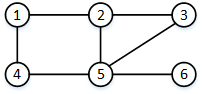
\includegraphics[height=0.8in] {figures/graph_G.png}
	}
	\caption{Graph $\mathbf{G_1}$, all edges' weight are $1$.}
	\label{fig:graph_G}
\end{figure}


\begin{figure}[ht]
	\centering
	\subfigure[]{
		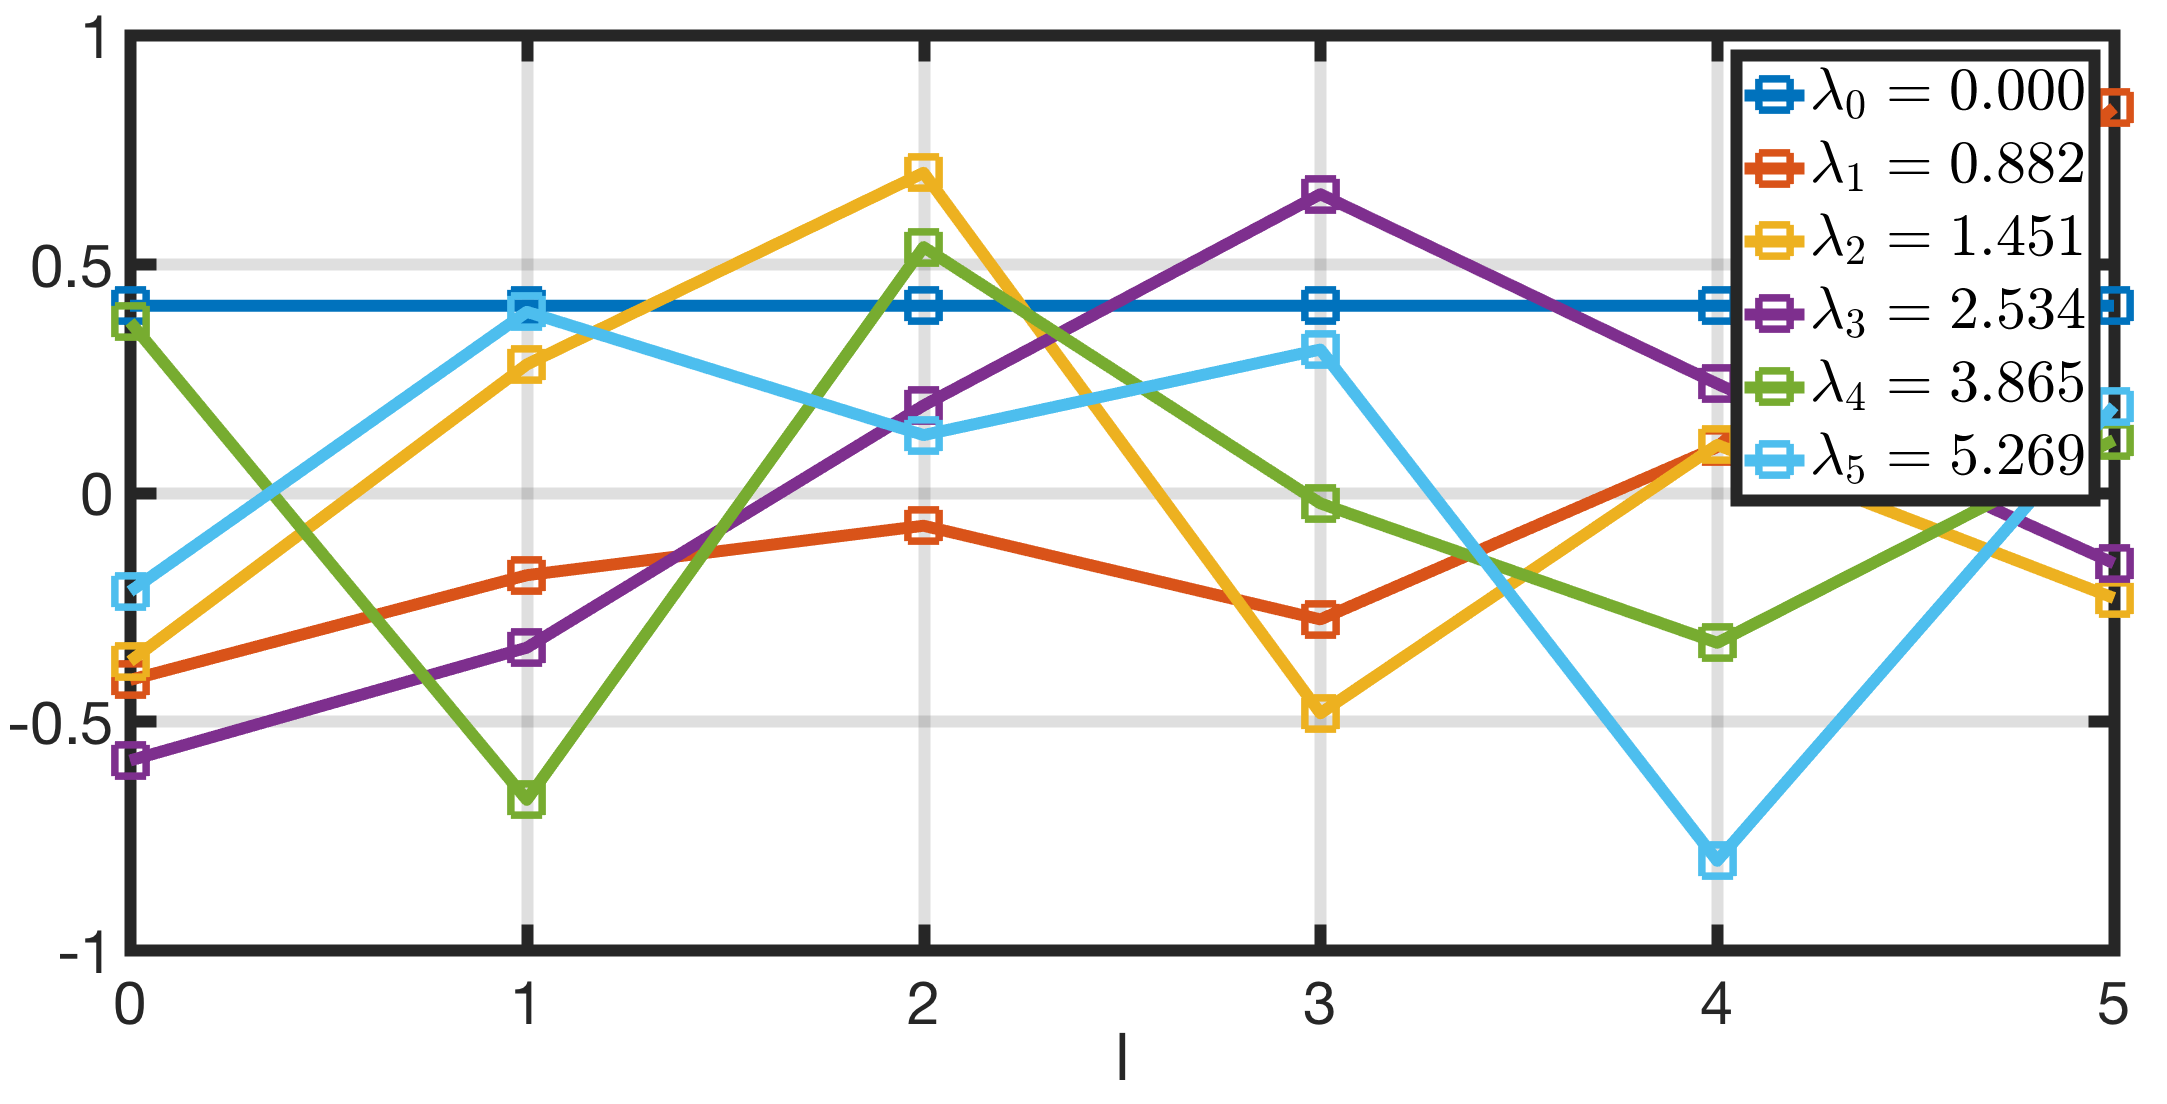
\includegraphics[width= 2.5in,height=1in] {figures/frequency.png}
		\label{fig:frequency1}
	}
	\subfigure[]{
		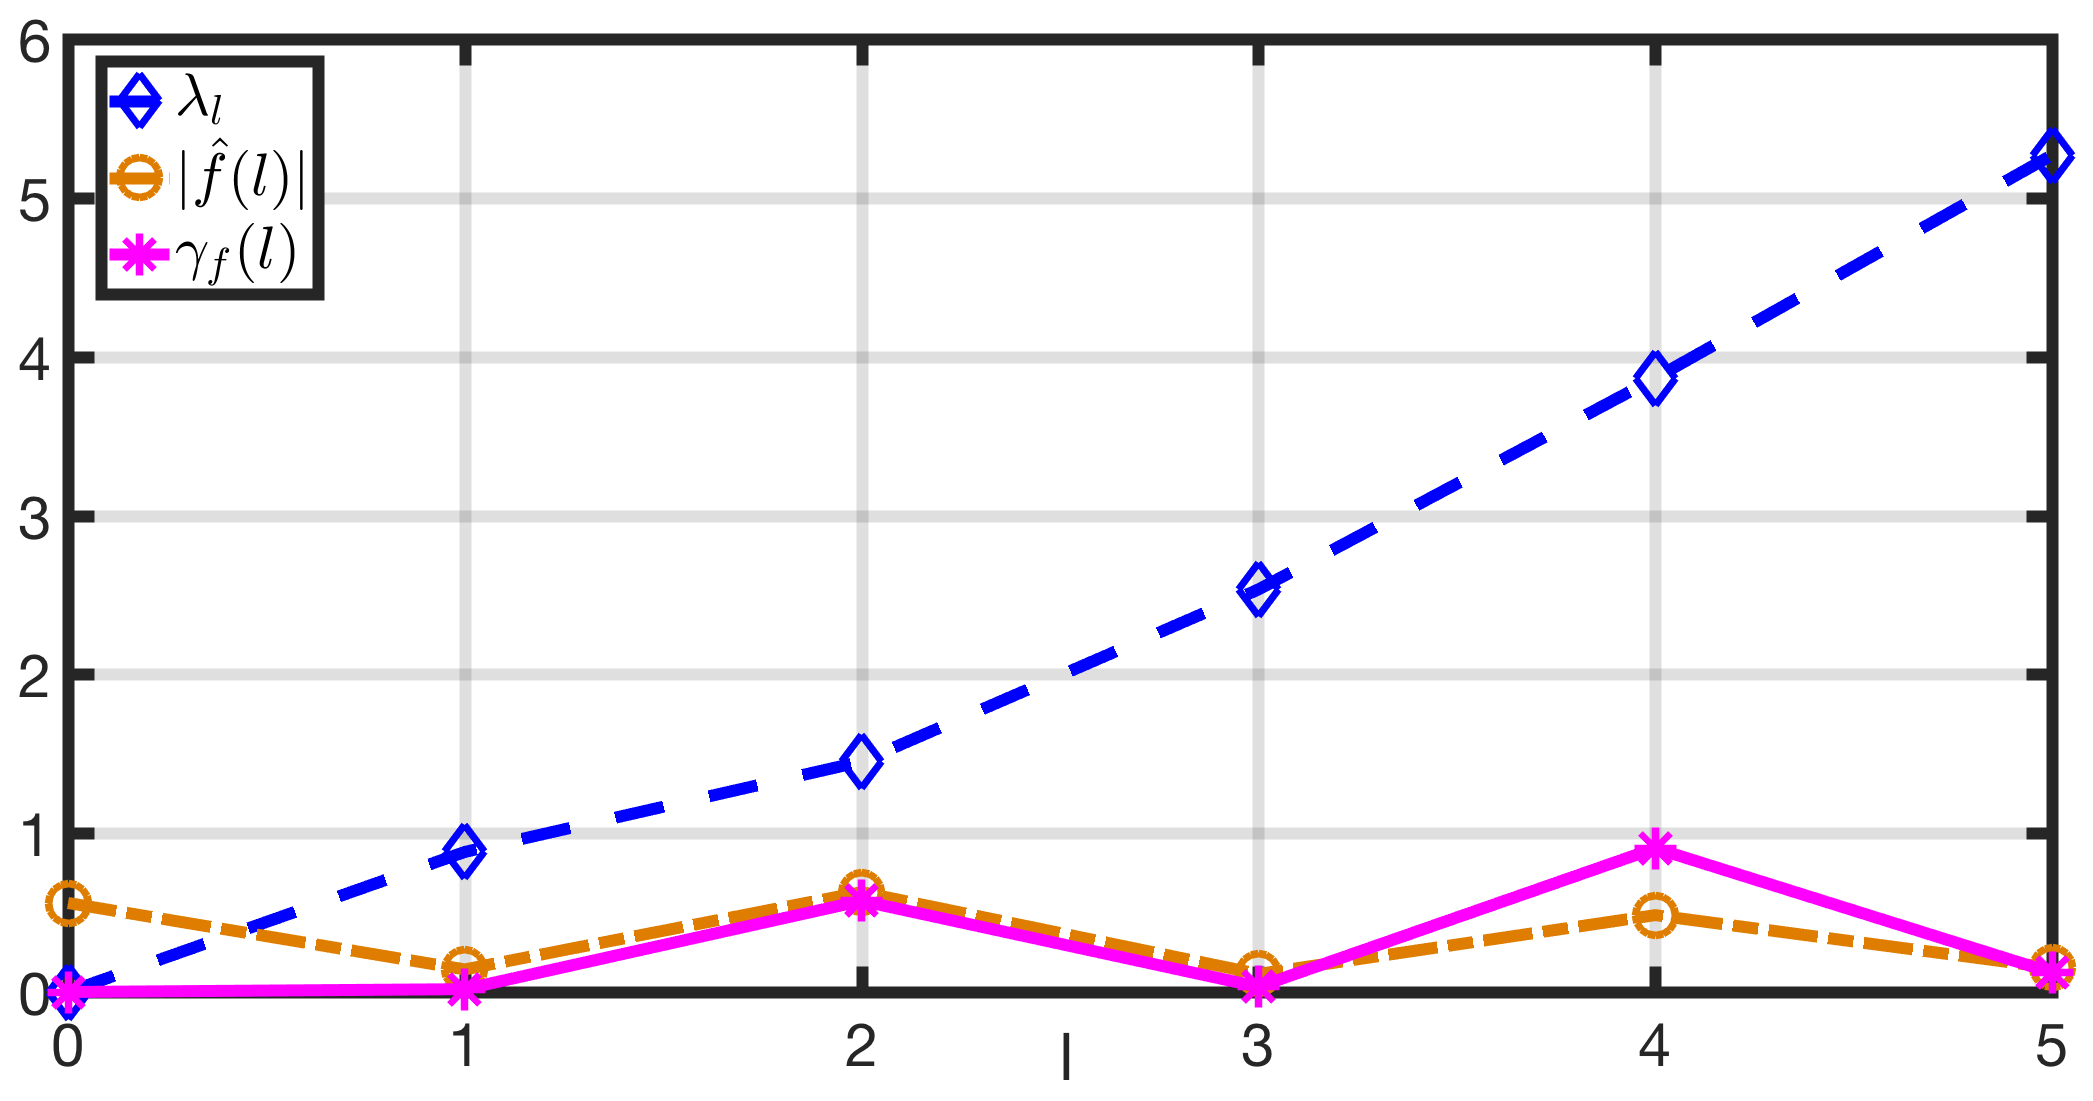
\includegraphics[width= 2.4in,height=1in] {figures/g1_gamma.png}
		\label{fig:g1_gamma}
	}

	\subfigure[]{
		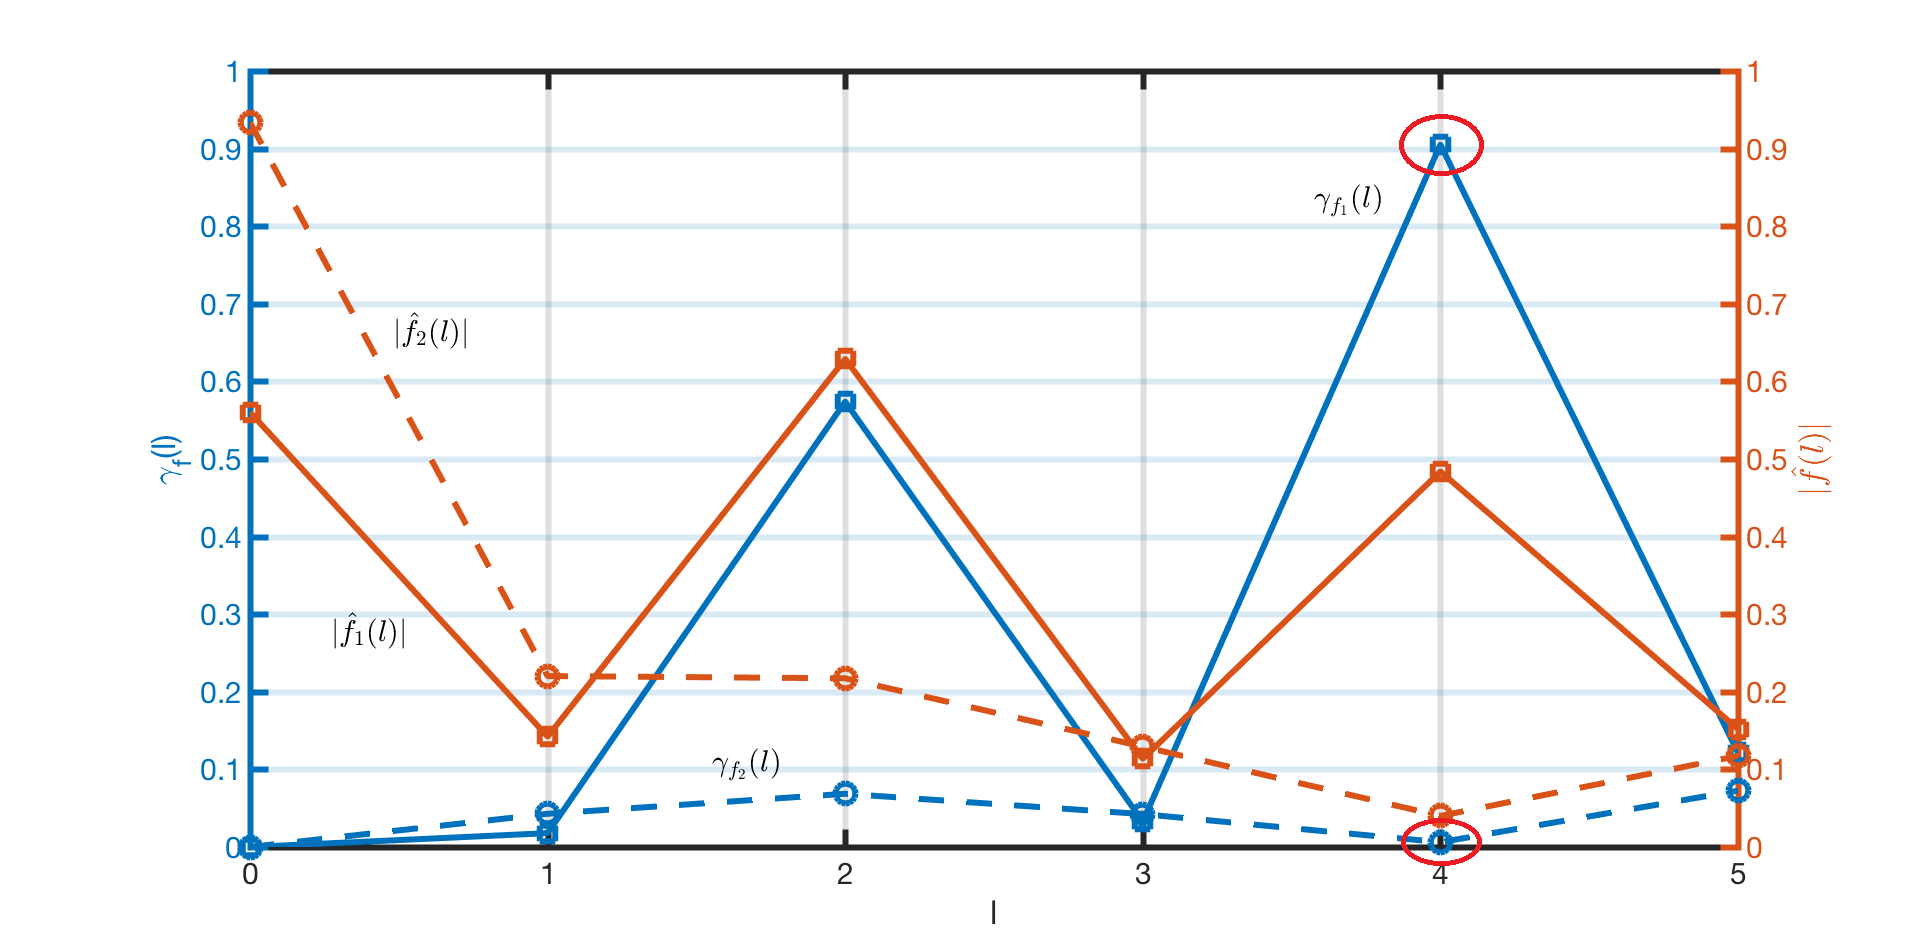
\includegraphics[width= 2.55in,height=1in] {figures/same_graph.png}
		\label{fig:same_graph}
	}

	\caption{(a): Eigenvector distribution along each vertex in graph $\mathbf{G_1}$.  (b): anomaly index $\gamma_f(l)$ of $f_1=[2,3,4,3,2,1]$ on graph $\mathbf{G_1}$. (c): anomaly index $\gamma_f(l)$ of $f_1=[2,3,4,3,2,1]$  and $f_2=[2,2,-3,4,3,1]$ on graph $\mathbf{G_1}$, where $\gamma_{f_1}=0.905$, and $\gamma_{f_1}=0.073$, labelled in red ovals.}
	\label{fig:f_on_g2}
\end{figure}

\subsection{Global Anomaly Index}
\label{sec:signal_anomaly_on_Graph}

To quantify the anomaly of a vector $f$ defined on a graph $\mathbf{G}$, it's necessary to incorporate the intrinsic structures of $\mathbf{G}$ and $f$. As discussed above, $\hat{f}(l)$ represents the coefficient of frequency $\chi_l$, and $\hat{f}^2(l)$ is considered as the energy of frequency $\chi_l$. In addition, according to equation~\ref{eq:lambda2}, $\lambda_l$ represents the deviation of frequency $\chi_l$ along all the connected vertices. Therefore, in this paper, we define the anomaly index of $\chi_l$ in $f$ as:
\begin{equation}
\label{eq:lambda3}
\gamma_f(l;\mathbf{G})=\lambda_l\hat{f}^2(l)= \lambda_l<f,\chi_l>^2
\end{equation}
$\gamma_f(l;\mathbf{G})$ depends on two parts, frequency $\chi_l$'s deviation sum $\lambda_l$, and its energy $\hat{f}^2(l)$. If the energy $\hat{f}^2(l)$ is small, even $\lambda_l$ is large, the anomaly index of $\chi_l$ might be small. Obviously, $\gamma_f(0;\mathbf{G})$ is always $0$ since $\lambda_0=0$. Further, we use the maximal value of $\gamma_f(l;\mathbf{G})$ to represent the global anomaly of $f$ on $\mathbf{G}$:
\begin{equation}
\label{eq:lambda4}
\gamma_f(\mathbf{G})=\underset{0 \leq l \leq N-1}{\max}{\gamma_f(l;\mathbf{G})}.
\end{equation}
Roughly speaking, $\gamma_f(l;\mathbf{G})$ means the anomaly extension of $\chi_l$ in $f$ defined on $\mathbf{G}$, instead of meaning anomaly extension of vertex $v_l$.
For brevity, $\gamma_f(l;\mathbf{G})$  and $\gamma_f(\mathbf{G})$ are shortened as $\gamma_f(l)$ and $\gamma_f$, respectively, when $\mathbf{G}$ is known.

Figure~\ref{fig:g1_gamma} plots the anomaly index $\gamma_f(l)$ of $f_1$ on graph $\mathbf{G_1}$, where $f_1=[2,3,4,3,2,1]$. The six markers on the dashed blue are the six eigenvalues of $\mathbf{G}$. The yellow line is $|\hat{f}(l)|$, and the pink line is the anomaly index, $\gamma_f(l)$ for frequency $\chi_l$. Because $\gamma_f(l)$ depends on both $\lambda_l$ and its power $\hat{f}^2(l)$, for the yellow line, even though $\chi_0$ has the strongest power, its deviation $\lambda_0 = 0$, thus $\gamma_f(0)=0$. On the other hand, $\chi_5$ has the largest deviation; but its power $|\hat{f}(5)|^2$ is small, which makes $\gamma_f(5)$ is also small. Considering $\chi_4$ has a high deviation (eigenvalue) and a strong power of frequency, thus $\chi_4$  has the largest anomaly index. To compare the influence of different $f$ on anomaly index, we show an example in Figure~\ref{fig:same_graph}. Set $f_1=[2,3,4,3,2,1]$ and $f_2=[2,2,-3,4,3,1]$, we plot their anomaly index $\gamma_{f}$ and energy $|\hat{f}(l)|$ respectively.
The light blue curves stands for anomaly index, and yellow curve stands for $|\hat{f}(l)|$. The solid line stands for $f_1$, and dashed line stands for $f_2$. As we can see, for high frequency $\chi_l$, $f_1$ has a larger power than $f_2$, and hence a higher anomaly index than $f_2$, where $\gamma_{f_1}=0.905$ and $\gamma_{f_2}=0.073$. This is consistent with that $f_1$ has larger deviations than $f_2$.

As we discussed before, the anomaly index depends on graph structure and $f$. As shown in Figure~\ref{fig:same_graph}, different $f$ might have very different anomaly index because the power of $\chi_l$ distribution is different. Similarly, for the same signal $f$ on two different graphs, it might have very different anomaly indices. Figure~\ref{fig:f_on_g} shows two graphs with the same $f=[1,2,5,2]$. Figure~\ref{fig:new_graph} illustrates the anomaly index of $f$ on $\mathbf{G_2}$ and $\mathbf{G_3}$, where $\gamma_{f}(\mathbf{G_2})=0.073$ and $\gamma_{f}(\mathbf{G_3})=0.235$. (This is because in $\mathbf{G_3}$ there is not edge connecting $v_2$ and $v_3$, the difference between $f(2)$ and $f(3)$ is not considered as anomaly.)


{\textbf{Remarks:}}
In this subsection, we introduce the anomaly index $\gamma_f(l;\mathbf{G})$ to measure the anomaly of $\chi_l$ in $f$ defined on $\mathbf{G}$ by combing the spectrum structure of $\mathbf{G}$ and $f$. $\gamma_f(l;\mathbf{G})$ depends on two parts: (1) the eigenvalue which reflects the deviations of $\chi_l$; (2) the $|\hat{f}(l)|^2$  which represents the power of $\chi_l$ in $f$. $\gamma_f(l;\mathbf{G})$ reflects the anomaly index of $\chi_l$. We use the maximal value of $\gamma_f(l;\mathbf{G})$ to define the anomaly index of $f$, which denotes the global anomaly index of $f$ on $\mathbf{G}$.



\begin{figure}[t]
	\centering
	\subfigure[$\mathbf{G_2}$]{
		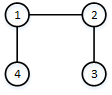
\includegraphics[height=0.8in] {figures/f_on_g1.png}
		\label{fig:scale1}
	}
	\subfigure[$\mathbf{G_3}$]{
		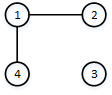
\includegraphics[height=0.8in] {figures/f_on_g2.png}
		\label{fig:scale2}
	}
	\caption{$f=[1,2,5,2]$ on two graphs $\mathbf{G_2}$ and $\mathbf{G_3}$.}
	\label{fig:f_on_g}
\end{figure}

\begin{figure}[h]
	\centering
    {
		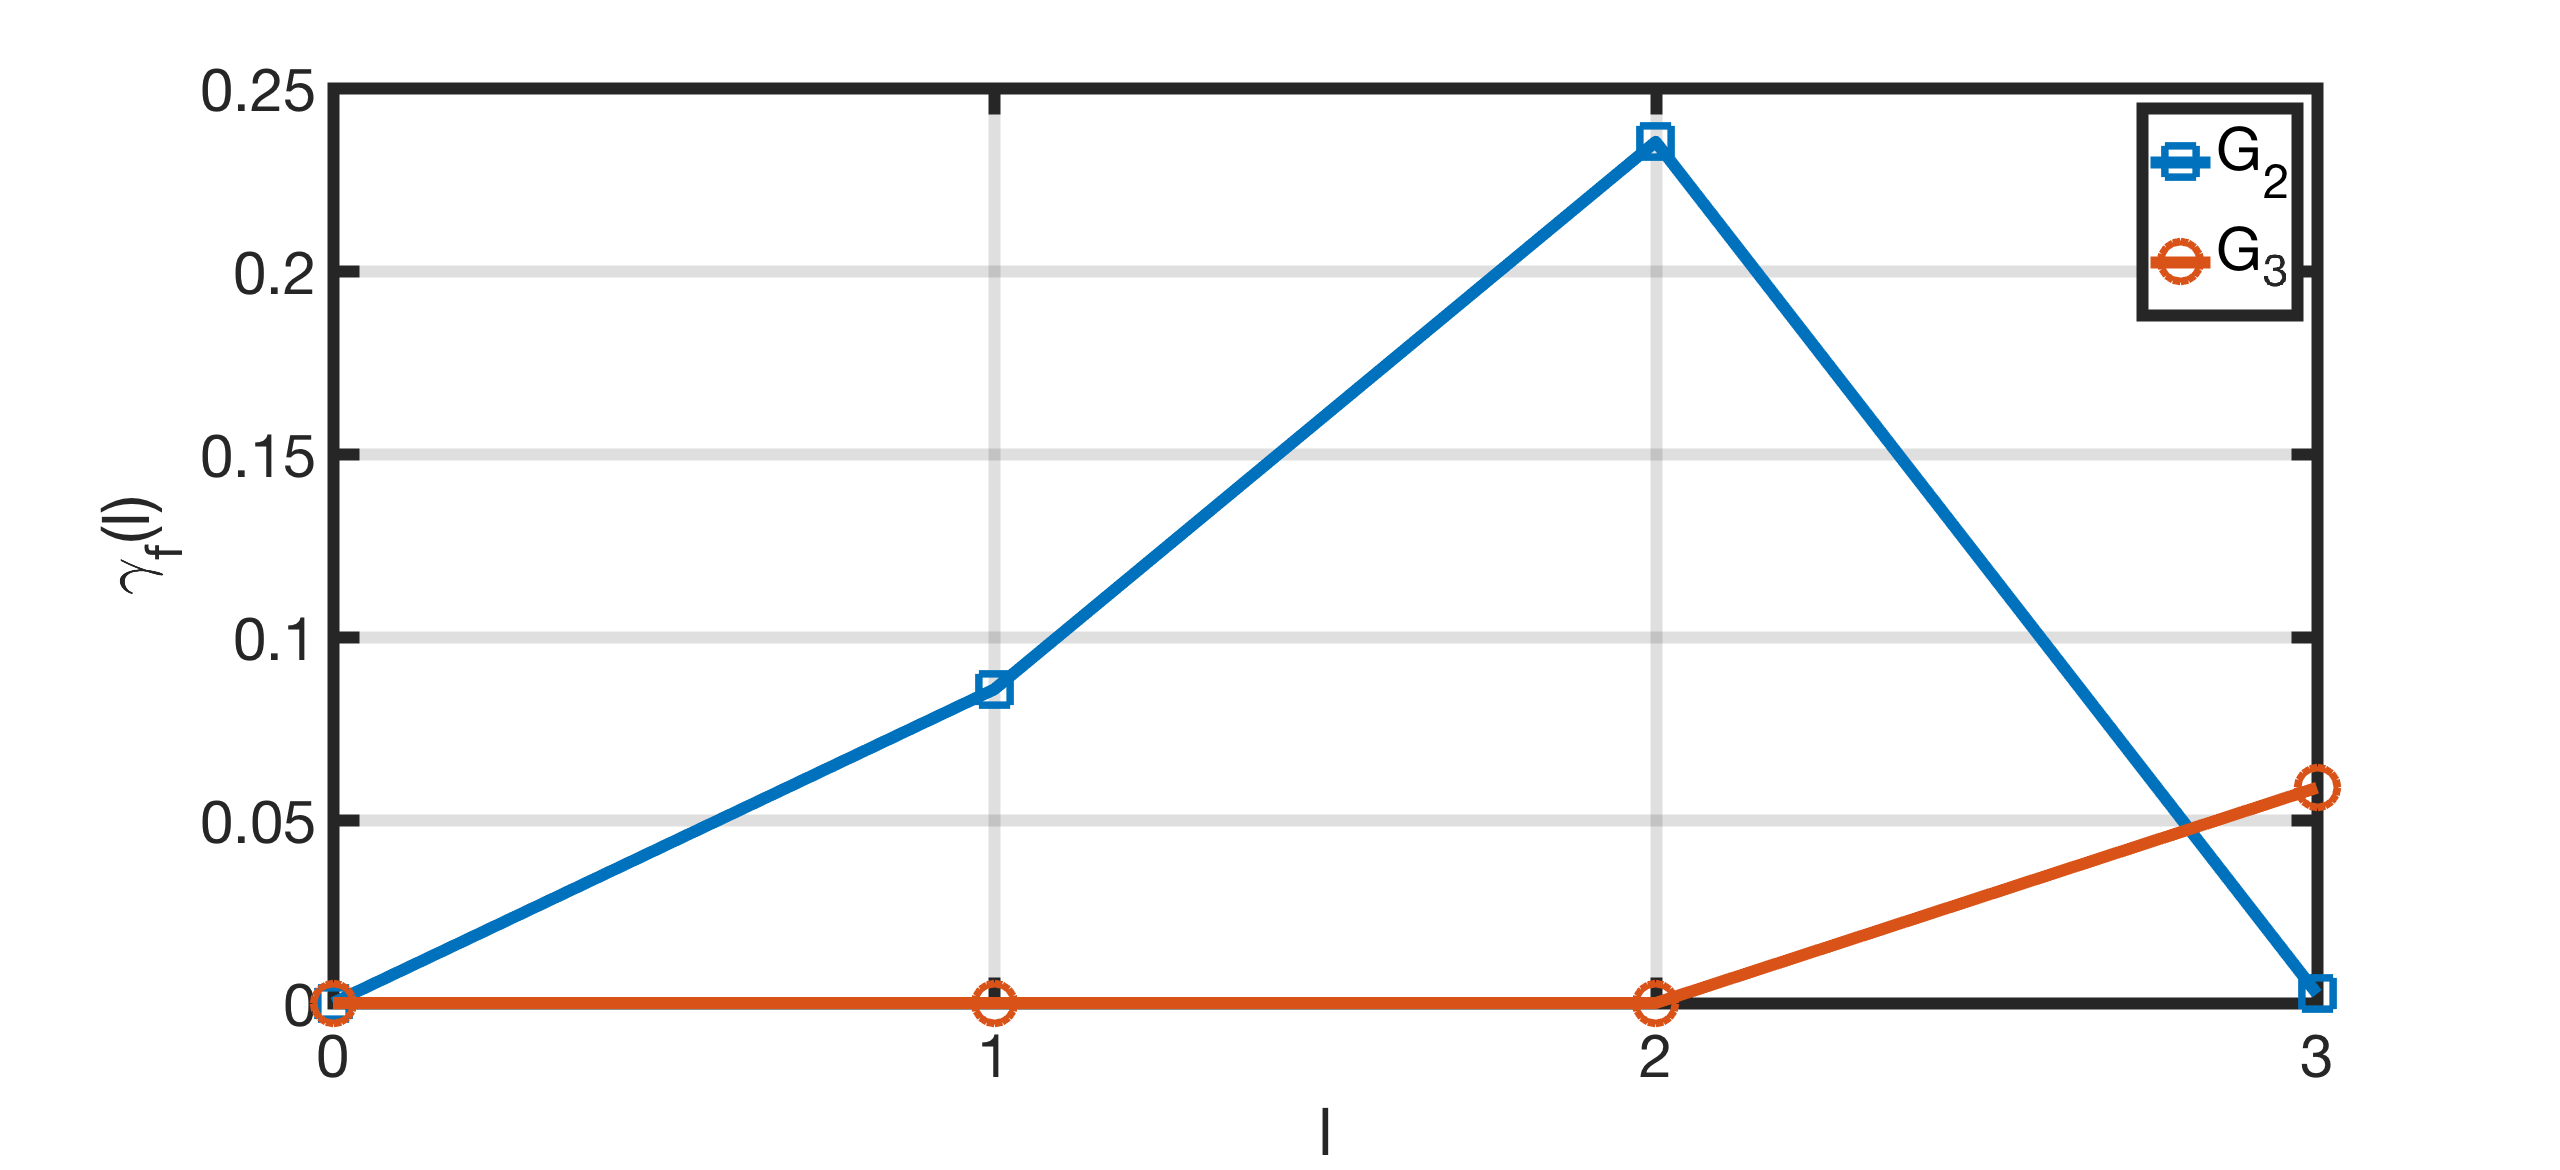
\includegraphics[width= 3.2in,height=1in] {figures/new_graph.png}
		\label{fig:distribution2}
	}
	\caption{Anomaly indices of $\mathbf{G_2}$ and $\mathbf{G_3}$.}
	\label{fig:new_graph}
\end{figure}


\subsection{Graph Wavelets}
\label{sec:graph_wavelet}
Classic wavelet is called mathematical microscope because of its capability of showing signal anomaly with different scales. In the case of complex networks, graph wavelets render the graph with good localization properties both in frequency and vertex (i.e. spatial) domains. Their scaling property allows us to zoom in/out of the underlying structure of the graph.

%It is useful to analyze $f$ by taking into account the intrinsic geometric structure of the graph $\mathbf{G}$. In order to identify and exploit structure of  $f\in \mathbb{R}^N$, the spectral graph $\sigma({\mathcal{L}}):=\{\chi_l\}_{l=0}^{N-1}$ can be used as a dictionary of atoms~\cite{shuman_ACHA_2013}. Thus, $f$ can be decomposed as a linear combination of $\{\chi_l\}_{l=0}^{N-1}$ as
%\begin{equation}
%\label{eq:graph_fourier}
%f(n)= \sum\limits_{l=0}^{N-1}\hat{f}(l)\chi_l(n)
%\end{equation}
%, where
%\begin{equation}
%\label{eq:graph_fourier1}
%\hat{f}(l):= \sum\limits_{n=0}^{N-1}\chi^*_l(n)f(n)
%\end{equation}
%$\chi_l$ is called the Fourier frequency of $f(n)$ based on the graph $\mathbf{G}$, and $\hat{f}(l)$ is the corresponding Fourier coefficient.
%Equation~\ref{eq:graph_fourier1} and Equation~\ref{eq:graph_fourier} are called Fourier transform and inverse Fourier transform, respectively.
%Equation~\ref{eq:graph_fourier1} gives a clear representation of the Fourier components in $f(n)$.

Recall from Equation~\ref{eq:Graph_Fourier_Transform1}, the anomaly pattern $\hat{f}(l)$ represents the anomaly components of $f$ from the whole graph prospective. However, information concerning the vertex-location can not be identified from the Fourier transform. To address this issue, Hammond et al.~\cite{hammond2011wavelets} proposed constructing wavelet transforms functions over the vertices using weighted graphs, described in the following steps:

\begin{enumerate}
\item Define a continuous generating kernel functions $g(x)$ on $\mathbb{R}^+$;
\item Then, select a central vertex $a \in {V}$ and scale $s$, set the frequency coefficients as $g(s\lambda_l)\chi^*_l(a)$ for each frequency component $\chi_l$;
\item Finally, sum up all those frequency components $\chi_l$.
\end{enumerate}
In this way, the graph wavelet at central vertex $a$ is constructed as:
\begin{equation}
\label{eq:graphwaveletdefinition}
\psi_{s,a}(n) = \sum\limits_{l=0}^{N-1}g(s\lambda_l)\chi_l^*(a)\chi_l(n)
\end{equation}
%After setting up the graph wavelet, the wavelet coefficients for $f$ can be defined as
%\begin{equation}
%\label{eq:graph_graphwavelet}
%W_f(s,a)=<\psi_{s,a}, f>=\sum\limits_{l=0}^{N-1}g(s\lambda_l)\hat{f}(a)\chi_l(n)
%\end{equation}
%\paragraph{\textbf{Properties}}
After setting up the graph wavelet, the wavelet coefficients for $f$ can be defined as
\begin{equation}
\label{eq:graph_graphwavelet}
W_f(s,a)=<\psi_{s,a}, f>=\sum\limits_{l=0}^{N-1}g(s\lambda_l)\hat{f}(a)\chi_l(n)
\end{equation}
Similar to classical wavelets, graph wavelets provide following three properties, which are presented in detail in~\cite{hammond2011wavelets}.
 \begin{enumerate}
 \item \textbf{Reconstruction.}
 When the kernel function $g(x)$ satisfies the admissibility condition and $g(0)=0$,  $f(n)$ can be reconstructed by the wavelet coefficients.
\item \textbf{Discretization and Wavelet Frames.} For practical applications, scale $s$ of graph wavelet $\psi_{s,a}$ should be sampled with a finite number of scales. Given a real valued function $h(x)$, satisfying
\begin{equation}
\hat{h}(\omega) = \sqrt{\int_\omega^\infty\frac{|\hat{g}(\omega')|^2}{\omega'}d{\omega'} },
\end{equation}
where $\hat{g}$ and $\hat{h}$ are the classical Fourier transform of $g(x)$ and $h(x)$, the scaling function $\phi_{a}(n)$ can be generated as:
\begin{equation}
\label{eq:graphscaledefinition}
\phi_{a}(n) = \sum\limits_{l=0}^{N-1}h(\lambda_l)\chi_l^*(a)\chi_l(n)
\end{equation}
Accordingly, the scaling coefficients are defined as
\begin{equation}
S_f(a)=<\phi_a,f>
\end{equation}
Using scale set $\Theta:=\{s_j\}_{j=1}^J$, the discretized graph wavelet set $\{\psi_{s_j,a}\}_{j=1}^{J}$ $_{a=0}^{N-1}$, and scaling function set $\{\phi_a\}_{a=0}^{N-1}$ constitute a frame~\cite{hammond2011wavelets}.
According to frame theory~\cite{daubechies1992ten}, $f\in \mathbb{R}^N$ can be reconstructed from those $NJ+J$ wavelet and scaling coefficients as
\begin{equation}
\label{eq:frame}
f(n)=\sum_{a=v_0}^{v_{N-1}}[\sum_{j=1}^{J}W_{f}(s_j,a)\psi_{s,a}(n)+S_f(a)\phi_{a}(n)].
\end{equation}For brevity, we assume that
\begin{equation}
\phi_a(n)=\psi_{s_0,a}(n),
\end{equation} and
\begin{equation}
S_f(a)=W_f(s_0,a).
\end{equation}Therefore, equation~\ref{eq:frame} can be written as
\begin{equation}
\label{eq:frame2}
f(n)=\sum_{a=v_0}^{v_{N-1}}\sum_{j=0}^{J}W_{f}(s_j,a)\psi_{s,a}(n).
\end{equation}In the later part of this paper, we do not differentiate scaling coefficient and wavelet coefficient, and call them both wavelet coefficient. A detailed algorithm and treatment concerning the choice of $\Theta$ can be found in~\cite{hammond2011wavelets}.


\begin{figure*}[t]
	\centering
	\subfigure[wavelet $\psi_{s_1,a}$]{
		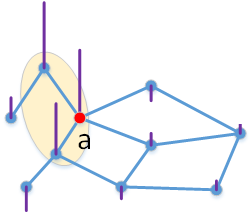
\includegraphics[width=1.4in, height=1.1in] {figures/wavelet1-2.png}
		\label{fig:scale1}
	}
	\subfigure[wavelet $\psi_{s_2,a}$]{
		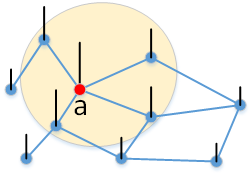
\includegraphics[width=1.4in, height=1.1in] {figures/wavelet2.png}
		\label{fig:scale2}
	}
\subfigure[$f(n)$ vs vertices]{
		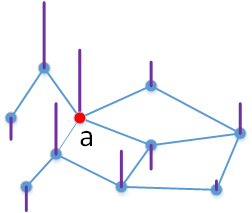
\includegraphics[width=1.4in, height=1.1in] {figures/wavelet3.png}
		\label{fig:scale3}
	}
\subfigure[$W_f(s,a)$ vs scale $s$]{
		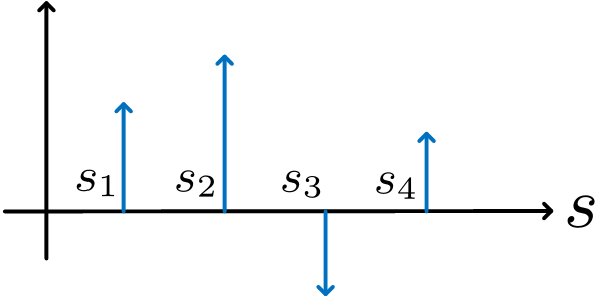
\includegraphics[width=1.5in, height=1.1in] {figures/wavelet4.png}
		\label{fig:scale4}
	}
	\caption{Graph wavelet scale and graph wavelet coefficient.}
	\label{fig:graphwaveletscale}
\end{figure*}




\item \textbf{Localization in vertex domains.} Given a central vertex $v_a$ and its graph wavelet $\psi_{s,a}(n)$, suppose the kernel function $g$ is $K+1$ times continuously differentiable, let $v_n$ be an vertex of $\mathbf{G}$ with $d_G(n,a)>K$, then there exists constants $D$ and $\beta$, such that
\begin{equation}
\label{equ:waveletbound}
\frac{|\psi_{s,a}(n)|}{||\psi_{s,a}||}\leq D \beta
\end{equation} for all $s<\beta$.
$d_G(n,a)$ is the shortest path distance, which is the minimum number of edges in any path that connect vertices $v_n$ and $v_a$~\cite{hammond2011wavelets}. Equation~\ref{equ:waveletbound} shows for any vertex $v_n$ that is far away from center vertex $v_a$ ($d_G(n,a)>K$), $\frac{|\psi_{s,a}(n)|}{||\psi_{s,a}||}$ is upper bounded by $D\beta$. In other words, for vertex $v_n$ which is far away form vertex $v_a$, its wavelet value is linearly attenuated by scale $s$.  When the scale $s$ is small, their wavelet value of marginal vertices will be vanished quickly. The marginal vertices are those which satisfy equation~\ref{equ:waveletbound}. All the other vertices are called kernel vertices, denoted by $\mathcal{K}(s,a)$. Obviously, $\forall v_n \in \mathcal{K}(s,a)$,  $d_G(n,a)\le K$. Thus $\mathcal{K}(s,a)$ is automatically compact.
Figure~\ref{fig:graphwaveletscale} shows two graph wavelets centered on the same vertex $a$, but with two different scales, $\psi_{s_1,a}$ and $\psi_{s_2, a}$, where $s_1<s_2$. The length of the vertical bar on each vertex denotes its graph wavelet value. The highlighted areas denote the kernel vertices ($d_G(n,a)\le 1$), and the others are marginal vertices. We can see that the wavelet values  on marginal vertices in Figure~\ref{fig:scale1} are smaller than those in figure \ref{fig:scale2}. Figure~\ref{fig:scale3} is $f$'s distribution along each vertex, and Figure~\ref{fig:scale4} shows the wavelet coefficients with center node $a$ for different scales, which indicates $W_f(s_2,a)$ has the largest value, and $W_f(s_3,a)$ has the smallest.
 \end{enumerate}
 
 

\subsection{Group Anomaly Detection via Graph Wavelet}
\label{sec:Group_Anomaly_Detection_via_graph_wavelet}
According to Equation~\ref{equ:waveletbound}, when $s$ is small, the weights of the marginal vertices are severely attenuated.
Essentially, $W_f(s,a)$ is equivalent to the sum of $f$ with large weights on kernel vertices, and small weights on marginal vertices.
%, and can also be treated as a similarity between $f$ and $\psi'_{s,a}$.
When $f$ is of uniformly large negative/positive values on kernel vertices, then $W_f(s,a)$ will be a large negative/positive value with scale $s$.

The localization property of graph wavelet makes it appropriate for group anomaly detection since it automatically identifies the kernel vertices from marginal vertices. These kernel vertices form a compact subset since each one of them is close to the same center vertex $a$, which avoids the compactness constrain condition in equation~\ref{eq: problem_conventional}, thus making its computational complexity greatly reduced. We propose our group anomaly detection algorithm based on graph wavelet, illustrated in Algorithm~\ref{algo:event_detection1}. It iterates $NJ+J$ times, and each iteration selects a vertex as the center node, and computes wavelet coefficient $W_f(s_j, a)$ with $J+1$ scales. When $W_f(s_j, a)$ is larger than some pre-set threshold $\omega_{th}$, it considers the corresponding kernel vertices, $\mathcal{K}(a)$, as abnormal burst group. Similarly, when $W_f(s_j, a)$ is smaller than $-\omega_{th}$, it considers $\mathcal{K}(a)$ as abnormal absenteeism group. The computational complexity is $O(J|V|^2)$.

\begin{algorithm}[ht]
\centering
\captionsetup{font=scriptsize}
\caption{Group Anomaly Detection Using Graph Wavelet}
{\footnotesize \begin{algorithmic}[1]
\STATE {\bf Input:} graph and absenteeism score vector $\mathbf{G}(V,E;f^l)$ at time interval $l$, wavelet threshold $\omega_{th}$.
\STATE {\bf Output:} abnormal burst group set $\mathcal{I}^{bur}$ and absenteeism group set $\mathcal{I}^{abs}$.	\STATE{compute graph spectrum $\sigma{(\mathbf{G})}$};
\STATE{set graph wavelets $\psi_{s,a}(n)$ and scales set $\{s_j\}_{j=0}^J$ for all $a\in V$};
\FORALL {center node $a\in V$ and $s_j \in \{s_j\}_{j=0}^J$}
	    \STATE{compute $W_f(s_j, a)$};
		\IF {$W_f(s_j, a) \ge \omega_{th}$}
		    \STATE{add group $\mathcal{K}(s_j,a)$ to $\mathcal{I}^{bur}$}
	    \ENDIF
	
		\IF {$W_f(s_j, a)\le -1*\omega_{th}$}
		    \STATE{add group $\mathcal{K}(s_j,a)$ to $\mathcal{I}^{abs}$}
	    \ENDIF	
	
\ENDFOR	
\RETURN {abnormal burst group $\mathcal{I}^{bur}$ and absenteeism group set $\mathcal{I}^{abs}$.}
\end{algorithmic}}
\label{algo:event_detection1}
\end{algorithm}


{\textbf{Remarks:}}
\begin{enumerate}
\item Graph wavelets form a frame, the function $f$ can be reconstructed by their coefficients.
As long as the scale level $J$ is high enough, $f$ can be well decomposed into the frame basis. Thus, using graph wavelets to exploit structure of functions defined on graphs is much more reasonable.
\item Graph wavelet transforms selected kernel vertices, $\mathcal{K}(s,a)$, that are close to the central vertex $a$, and attenuate the impact of other marginal vertices that are far away from $a$. The abnormal group selected by graph wavelet approach is automatically compact, and circumvent high computational complexity, which makes is easily adaptable to a wide variety of application scenarios.
\item Graph wavelet is able to identify abnormal burst group and absenteeism group simultaneously without extra computation cost.
\end{enumerate}


\begin{figure}[th]
	\centering
	\subfigure[wavelet $\psi_{s_1,a}$]{
		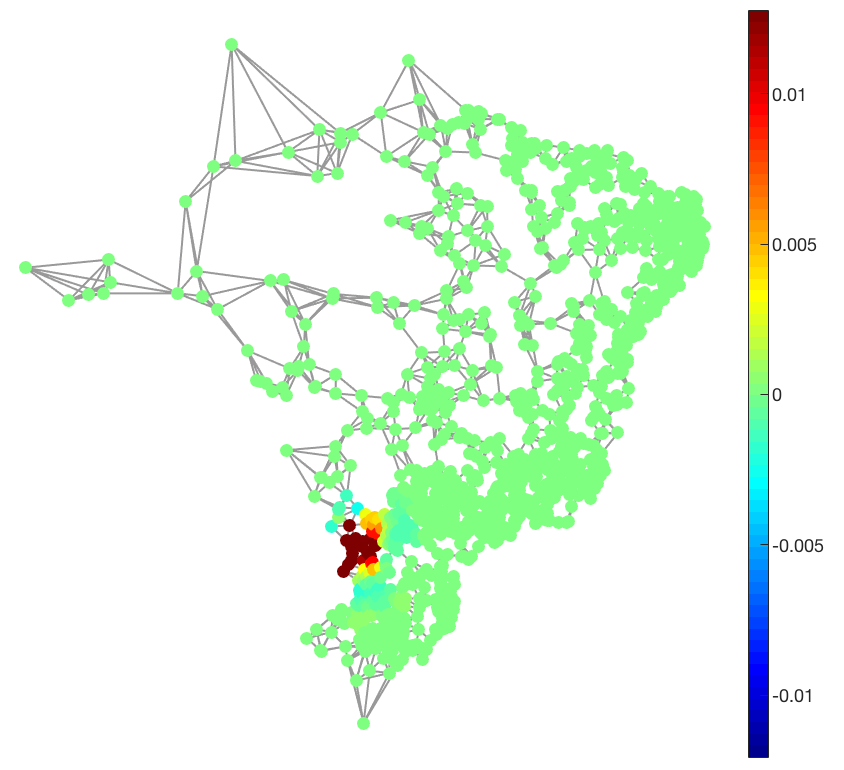
\includegraphics[width=1.3in] {figures/s1.png}
		\label{fig:Brazil_W_coeff_date31_s3}
	}
	\subfigure[wavelet $\psi_{s_2,a}$]{
		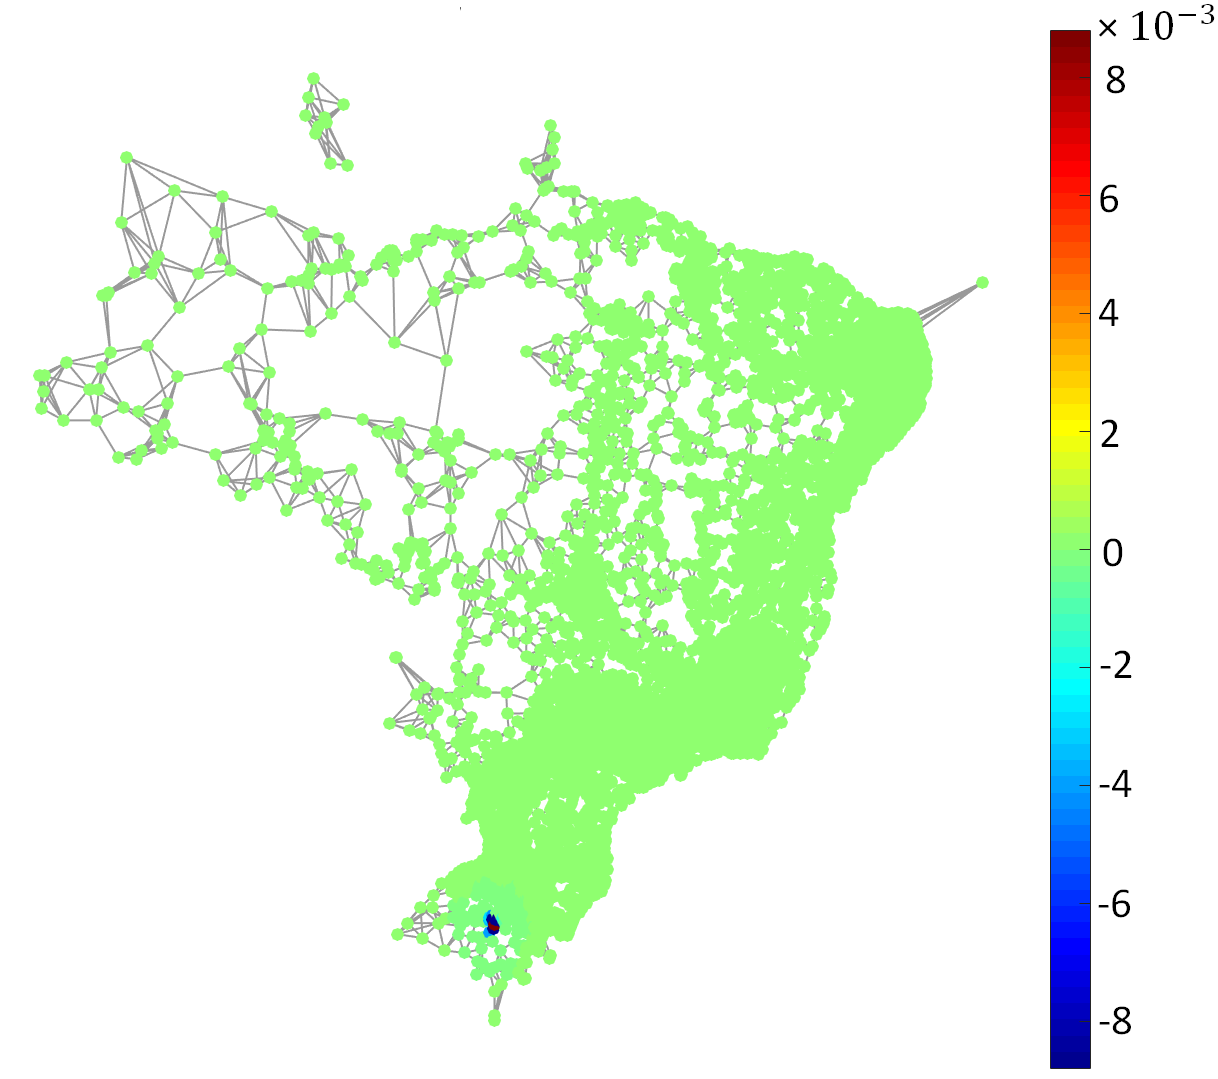
\includegraphics[width=1.3in] {figures/s2.png}
		\label{fig:Brazil_W_coeff_date31_s5}
	}
	\caption{Graph wavelets with center city $v_{83}$. $s_1$ = 1.31, $s_2$ = 0.68.}
	\label{fig:graphwaveletscale}
\end{figure}





\begin{figure}[th]
	\centering
	\subfigure[$W_f(s_1,a)$]{
		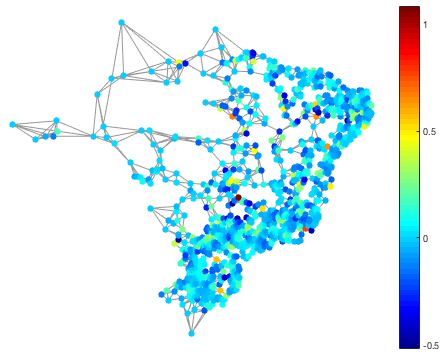
\includegraphics[width=1.3in] {figures/Brazil_W_coeff_date31_s3.png}
		\label{fig:Brazil_W_coeff_date31_s3}
	}
	\subfigure[$W_f(s_2,a)$]{
		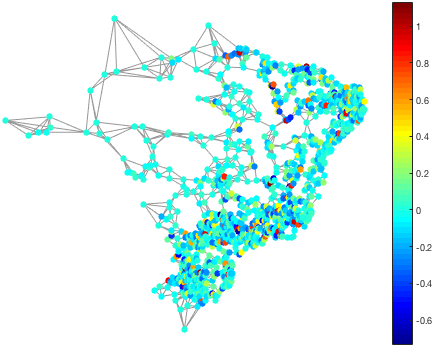
\includegraphics[width=1.3in] {figures/Brazil_W_coeff_date31_s5.png}
		\label{fig:Brazil_W_coeff_date31_s5}
	}
	\caption{Graph wavelet coefficient $W_f(s_1,a)$ and $W_f(s_2,a)$.}
	\label{fig:graphwaveletcoefficient}
\end{figure}





\section{EXPERIMENTAL RESULTS}
\label{sec:experiment}
This section discusses the applications of our approach for detecting group anomaly.
We begin by briefly describing the dataset we used for our experiments in Section~\ref{sec:data_collection}.
Then we discuss in Section~\ref{sec:experimental_setup} the implementation details of how we assemble the graph $\mathbf{G}$ and construct the graph wavelets $\psi_{s,a}$.
After that, we present group anomaly detection performance in protest events detection. In Section~\ref{sec:highlighted_results}, we describe three case studies that illustrate how the graph wavelet is able to capture absenteeism events like disaster scenarios.


\subsection{Data Collection and Preprocessing}
\label{sec:data_collection}
The study described in this paper uses Tweets in Latin America that were collected over 2 years (Jan 2012 to June 2014).
We query Datasift's streaming API to collect these Tweets that also have meta-information including geotag bounding boxes (structured geographical coordinates), Twitter Places (structured data), user profile location (unstructured, unverified strings), and `mentions information' about locations present in the body of the Tweet.
Typically, we found the number of Tweets with readily available geo-coordinates is too low for conducting meaningful experiments.
To circumvent this, we use the geo-enrichment algorithm described in~\cite{ramakrishnan2014beating}.
This algorithm uses a gazetteer-based approach to look-up location names and geo-coordinates.
To identify location-specific Tweets, we configure the geocoding tool to first consider the Tweet's text for mentions of place names and geographical landmarks (e.g., say, Plaza de la Independencia (Quito, Ecuador)).
In cases when no geographical location was found in the Tweets text, it then proceeds to process the geographical coordinates and the self-reported location string in user's profile metadata.
Using the geocoding tool, we were able to extract Tweets corresponding to $598,300$ unique cities from Latin America.

%To prepare a dataset of ground truth events for our study, we focused on specific types of disruptive societal events, such as natural disasters.
%We assume that such events are the predominant reasons that can cause group absenteeism on social networks.
%To discern when major events occurred, we retrieved records of natural disaster related events involving earthquakes, floods, and landslides from European Emergency Response Coordination Center(ERCC)~\footnote{http://erccportal.jrc.ec.europa.eu/} and World Top Stories Timeline~\footnote{http://www.mapreport.com/}.



\subsection{Experimental Setup}
\label{sec:experimental_setup}

\paragraph{Graph Setup}
Each city $v_i$'s location is represented by its geographical coordinate pair $lat_i$ and $lon_i$. Instead of using the real physical distance, we define the distance of any two cities $v_i$ and $v_j$ as $d_{ij}=\sqrt{(lat_i-lat_j)^2+(lon_i-lon_j)^2}$. We setup graph $G$ as a $k$ neighbors graph, which means  each city is only  connected to its $k$-nearest-neighbors. In this paper, we set $k=5$, and all the edges' weights  in $G$ are 1. Figure~\ref{fig:brazil_graph_nn_5} shows Brazil' $5$ nearest-neighbor Graph with 5321 cities.

\begin{figure}[t]
	\centering
	\subfigure[]{
		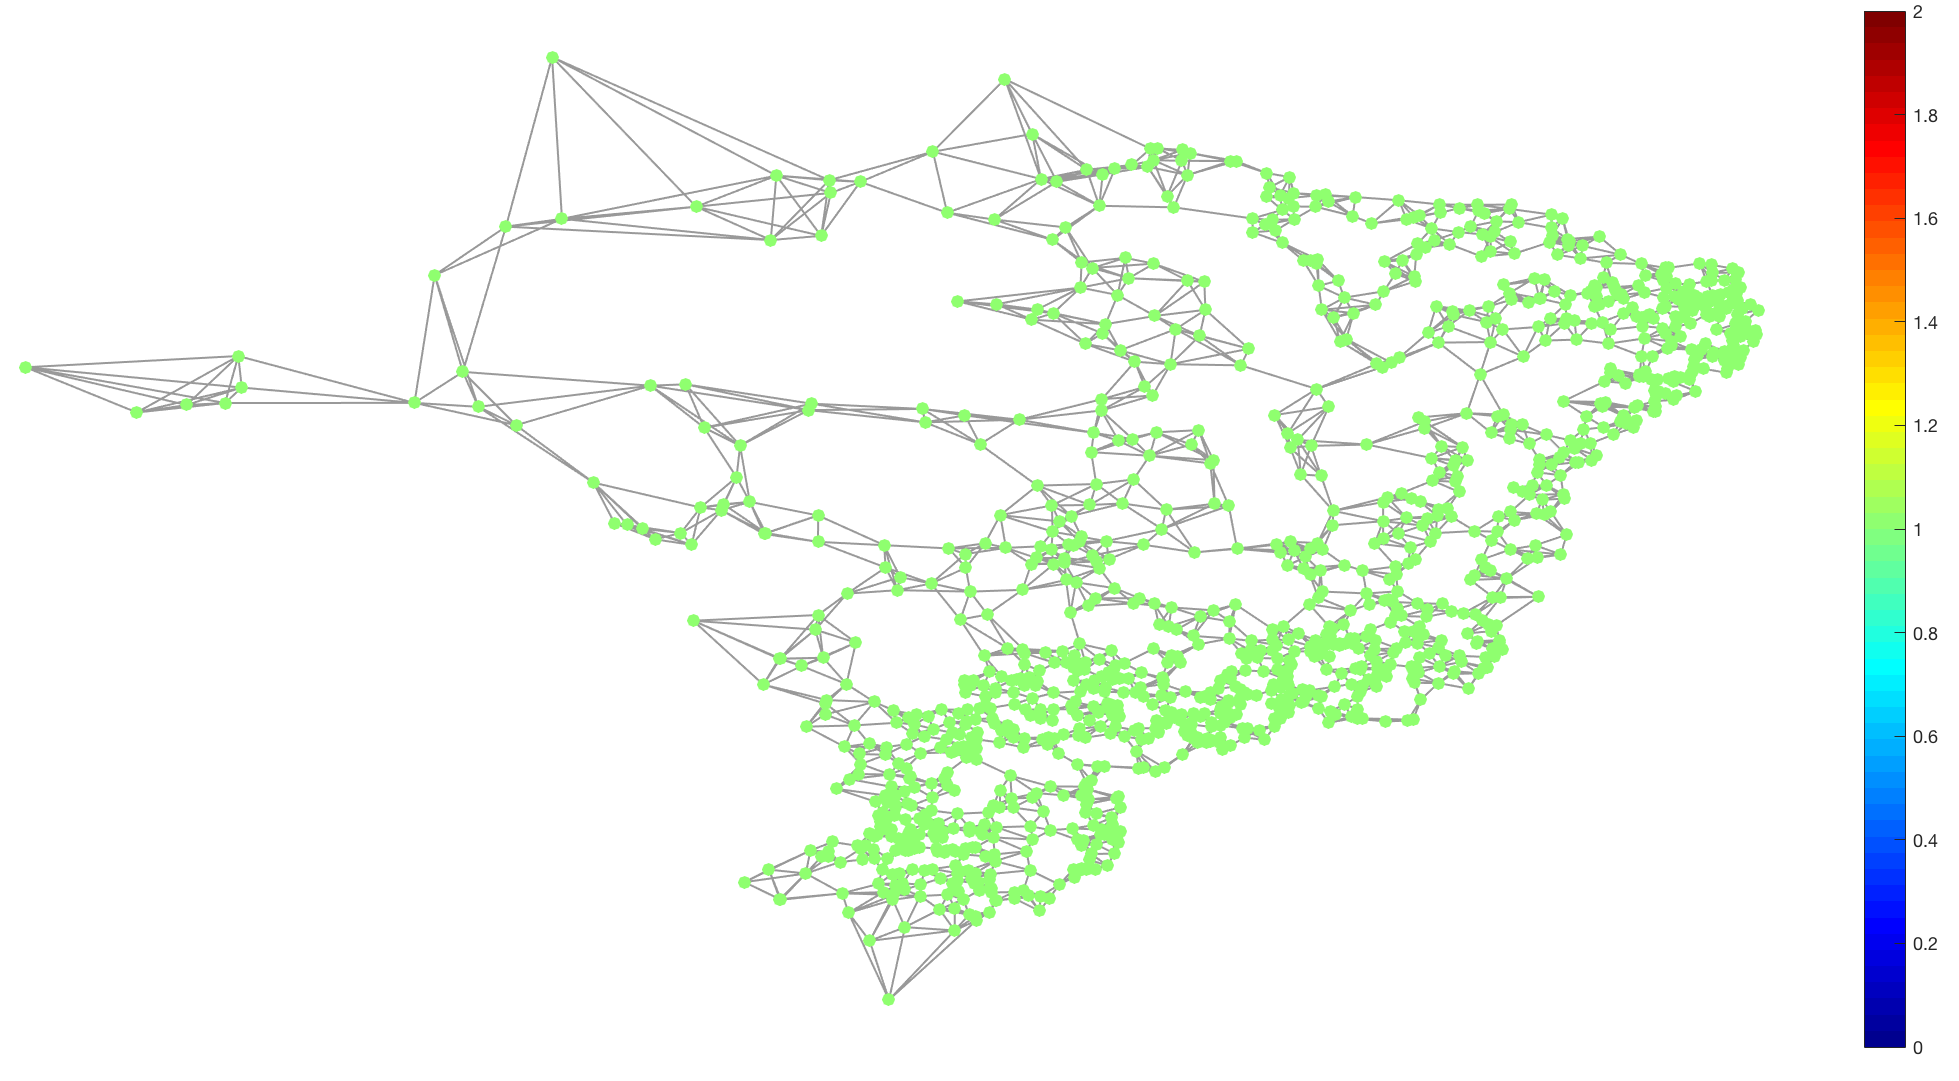
\includegraphics[width=1.5in,height=1.2in] {figures/brazil_graph_nn_5.png}
		\label{fig:brazil_graph_nn_5}
	}
	\subfigure[]{
		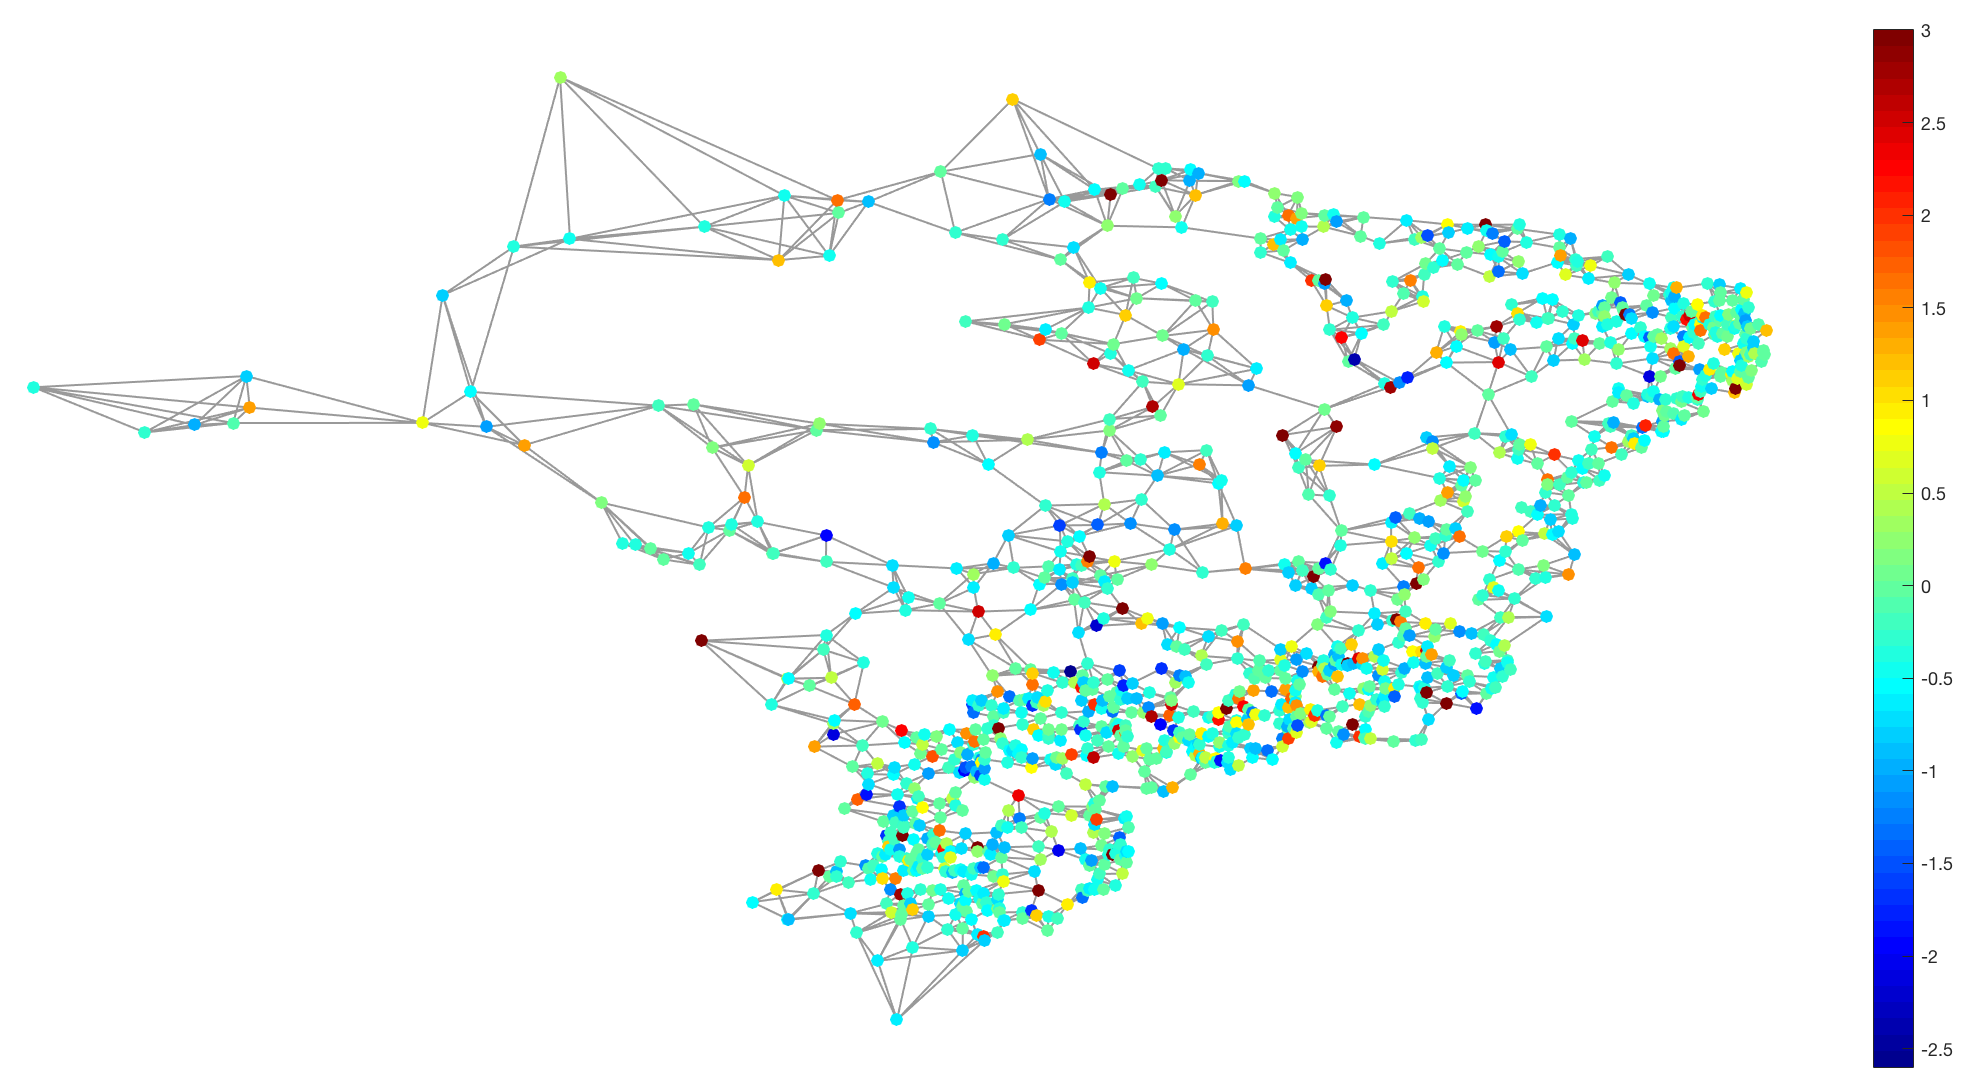
\includegraphics[width=1.5in,height=1.2in] {figures/brazil_zscore_31.png}
		\label{fig:brazil_zscore_31}
	}
	\caption{(a) Brazil's 5-nearest-neighbor Graph: 5321 cities, all edges' weights are $1$. (b) Brazil's Z-score distribution on July 31th, 2013. The color bar shows the scale of Z-score.}
	\label{fig:knn_zscore}
\end{figure}



\paragraph{Absenteeism Score}
Considering the Tweets volume $X$ varies vastly among cities, instead of using $X$ itself, we use the normalized value Z-score as absenteeism score, which is defined as:
\begin{equation}
\label{eq:Z_score}
Z-score= \frac{X-\mu}{\sigma}
\end{equation}Where, $\mu$ is the mean value of the previous $30$ days Tweets volume, and $\sigma$ is the corresponding standard deviation. As shown in Figure~\ref{fig:brazil_zscore_31}, different node color shows cities' different Z-score value.

\paragraph{Kernel function $g(x)$ and scaling function $h(x)$}
Our choice for the wavelet generating kernel function, $g(x)$, and scaling function $h(x)$ is motivated by our goal to achieve scale-dependent localization. We set $g(x)$ and $h(x)$ as:
\begin{equation}
g(x) = \left\{ \begin{array}{rl}
 x &\mbox{ for $x<1$} \\
s(x) &\mbox{ for $1\leq x \leq 2$} \\
 2x^{-1} &\mbox{ for $x>2$} \\
       \end{array} \right.
\end{equation} where $s(x)=-5+11x-6x^2+x^3$.
\begin{equation}
h_{x}= 1.385*exp(-(\frac{20x}{0.6\lambda_{max}})^4)
\end{equation}
The scale set $\{s_j\}_{j=1}^J$ is selected to be equally logarithmically spaced between the minimum and maximum scales $s_1$ and $s_J$, which are defined in~\cite{hammond2011wavelets}. We set $J=6$ in the experiment.

\paragraph{Anomaly index $\gamma_f(G)$ and $\omega_{th}$}
We claim that the event frequency $\eta$ is linear to $\gamma_f(\mathbf{G})$, described as
\begin{equation}
\label{eq:linear_equation}
\eta = k_0*\gamma_f(\mathbf{G}) + k_1
\end{equation}We use historical data to train $k_0$ and $k_1$ by least square error criterion. Once we know
$k_0$ and $k_1$, given a new $\gamma_f'(\mathbf{G})$, the events number is estimated as $m=\left \lceil \eta' \right \rceil$. After that the threshold $\omega_{th}$ is set as the $m$ largest $W_f(s_j,a)$, for all $a\in V$, $0\le j \le J$.




\begin{table}[bt] %!htp
\renewcommand{\arraystretch}{1.1}
\caption{\label{table:models_compare} The performance of graph wavelet vs. baseline and Z-score.}
\scriptsize
\centering
\begin{tabular}{ l | l |l | l | l}
\hline
\textbf{Country} & \textbf{Method}& \textbf{Precision}  & \textbf{Recall}  & \textbf{F-measure} \\
\hline
Brazil & Baseline & 0.052 &0.104 & 0.060\\
       & Z-score & 0.117&0.307 & 0.159 \\
 & Graph wavelet& 0.404 &0.262 & 0.292 \\
\hline
Mexico & Baseline & 0.074 &0.124 & 0.090 \\
       & Z-score & 0.221 &0.147 & 0.168 \\
 & Graph wavelet& 0.397 &0.384 & 0.408 \\
\hline
Venezuela & Baseline & 0.078 &0.053 & 0.059 \\
       & Z-score & 0.197 &0.197 & 0.189 \\
 & Graph wavelet& 0.292 &0.554 & 0.355 \\
\hline
\end{tabular}
\end{table}


\begin{figure}[t]
	\centering
	\subfigure[Brazil]{
		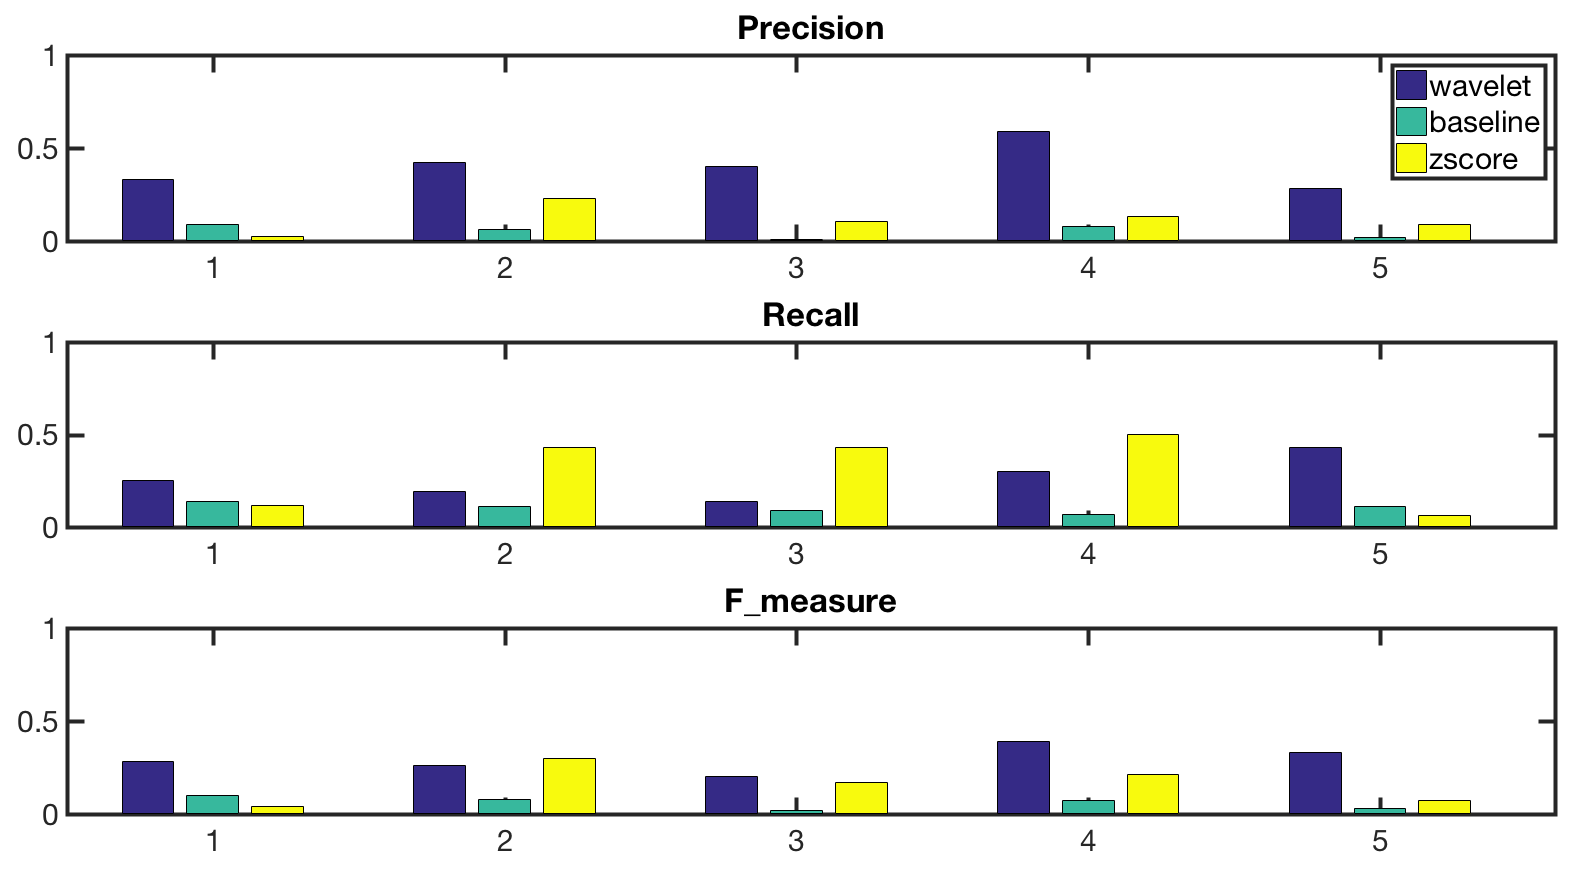
\includegraphics[width= 2.6in,height=1.4in] {figures/performance_compare_bar_graph_brazil.png}
		\label{Brazil_performance}
	}
	\hfill
	\subfigure[Mexico]{
		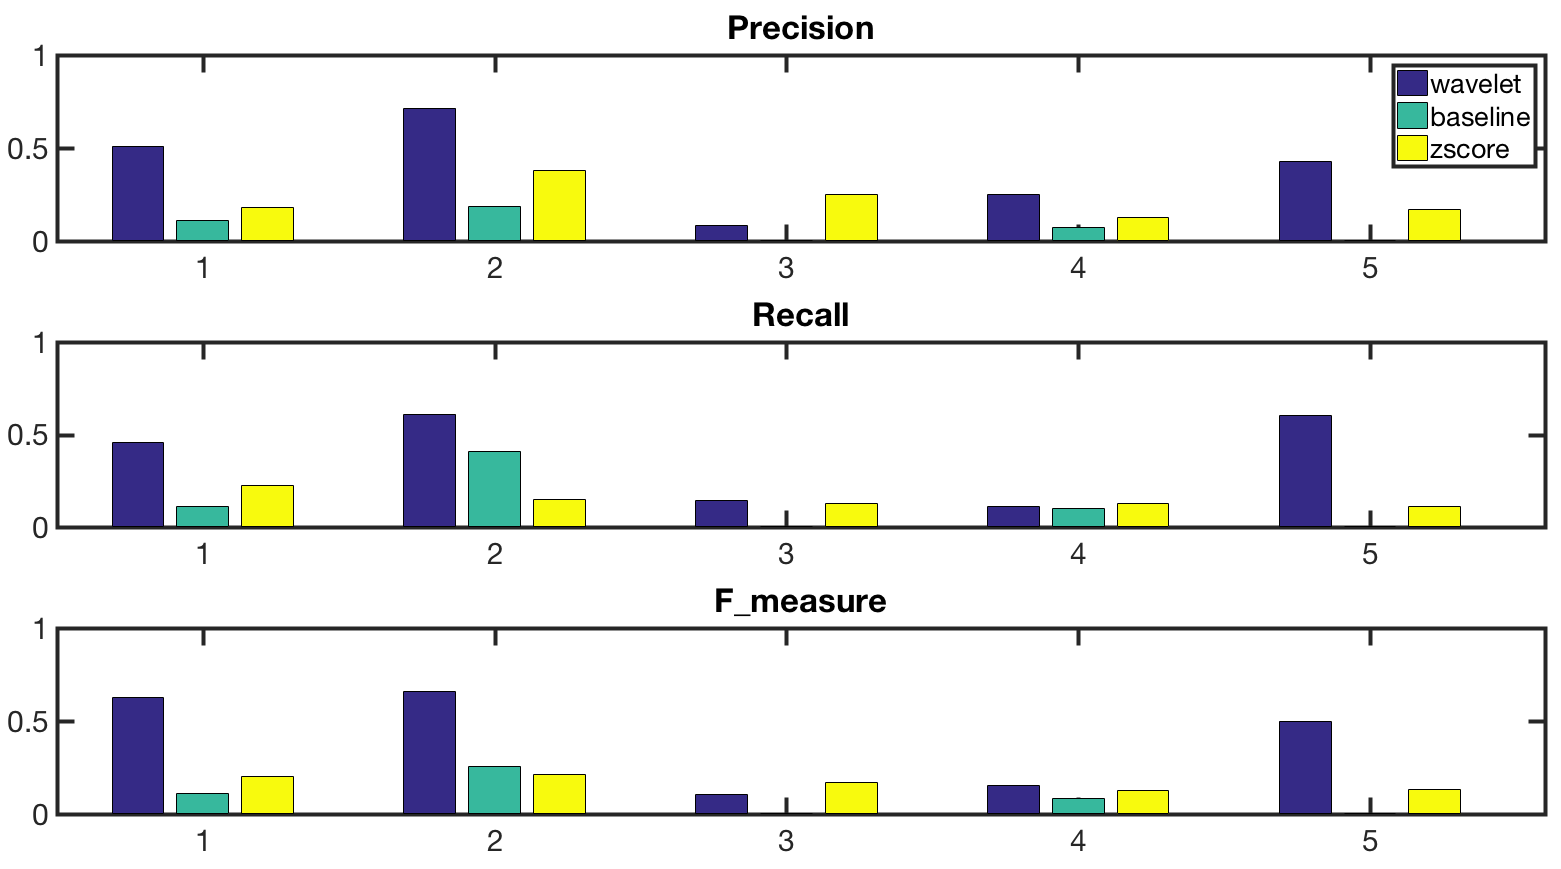
\includegraphics[width= 2.6in,height=1.4in] {figures/performance_compare_bar_graph_mexico.png}
		\label{Mexico_performance}
	}
	\hfill
	\subfigure[Venezuela]{
		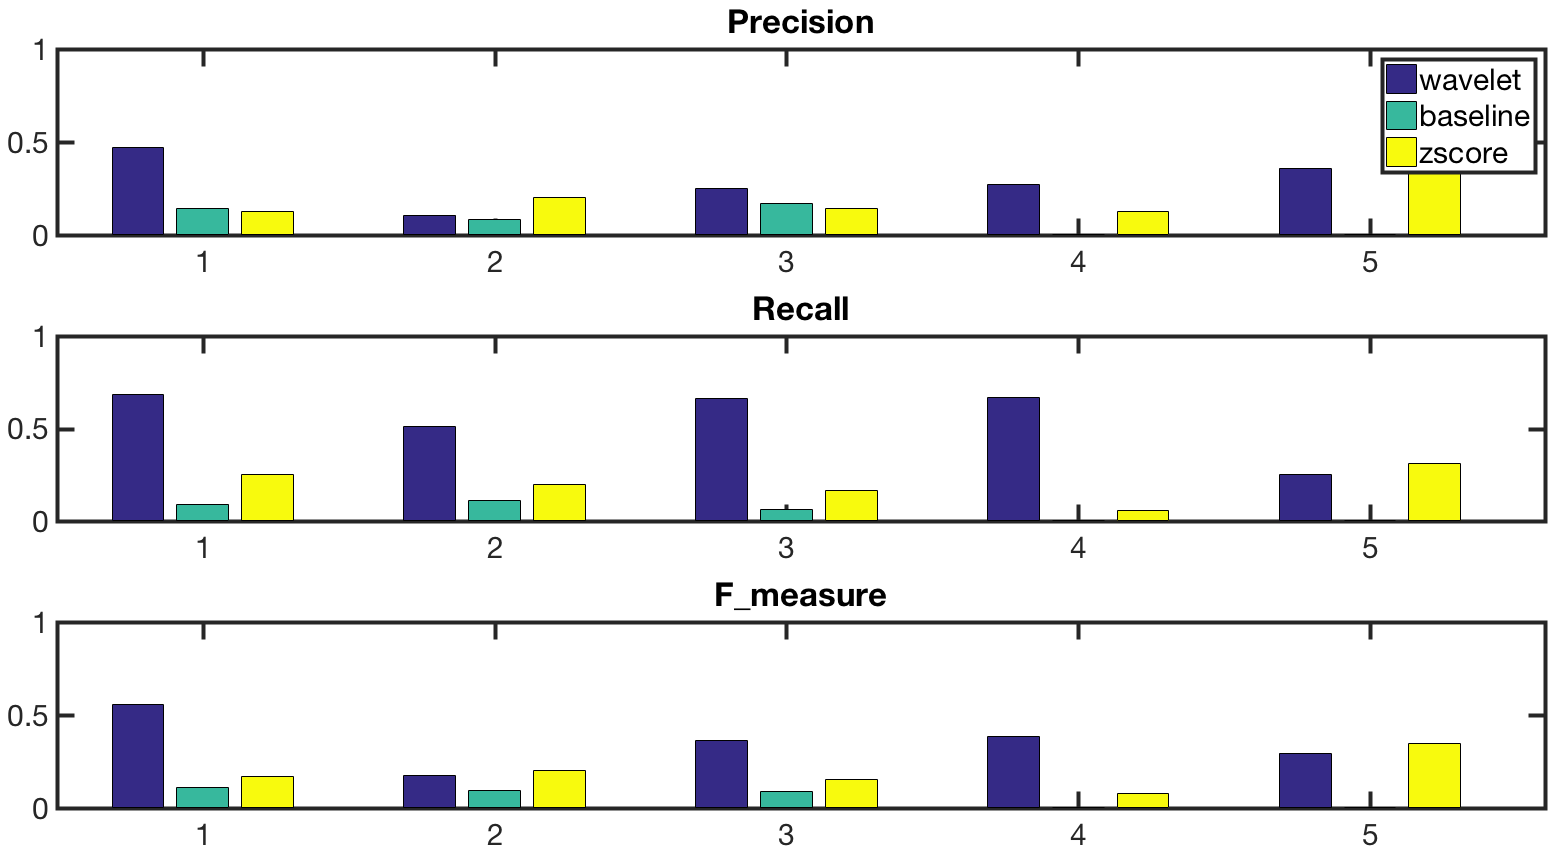
\includegraphics[width= 2.6in,height=1.4in] {figures/performance_compare_bar_graph_venezuela.png}
		\label{Venezuela_performance}
	}
	\caption{Brazil, Mexico and Venezuela protest detection performance.}
\label{fig:threecountry_performance}
\end{figure}


\subsection{Performance}
We did experiment on three major protest countries: Brazil, Mexico and Venezuela, from Jan 2013 to Dec 2014. Taken the Gold Standard Report (GSR)~\cite{ramakrishnan2014beating} as grand truth, we run the group anomaly detection algorithm. For each day, decide whether there is any anomaly, if there is, identify the group of abnormal cities, then compare with GSR, see if the selected cities have protest events on that day, how many of them are matched with grand truth, how many of them do not have protest. We use recall, precision and F-measure to evaluate the performance.
To evaluate our performance, we also compare with some intuitive approaches, like frequency based random assignment, we call it baseline model, and Z-score based selection methods. The baseline model is built according to the historical protest records of each city, based on frequency, predict the future protests occurrence. The Z-score approach is, selecting the group of cities whose Z-score across some threshold, say $|Z-score|>3$.

We compare three models' performance over two years period, and show the overall results on Table~\ref{table:models_compare}. Generally speaking, graph wavelet has the best precision, recall, and F-measure than baseline across countries. The mean F-measure for graph wavelet detection across models and countries is greater than other models. Interestingly, we find that the graph wavelet work at different efficiency levels depending on country. From Figure~\ref{fig:threecountry_performance}, we found graph wavelet model has a much higher recall in Venezuela than in Brazil, while has an inferior quality of event detection in Mexico than in Venezuela.

\subsection{Case Studies}
\label{sec:highlighted_results}

\begin{figure}[t]
	\centering
	\subfigure[]{
		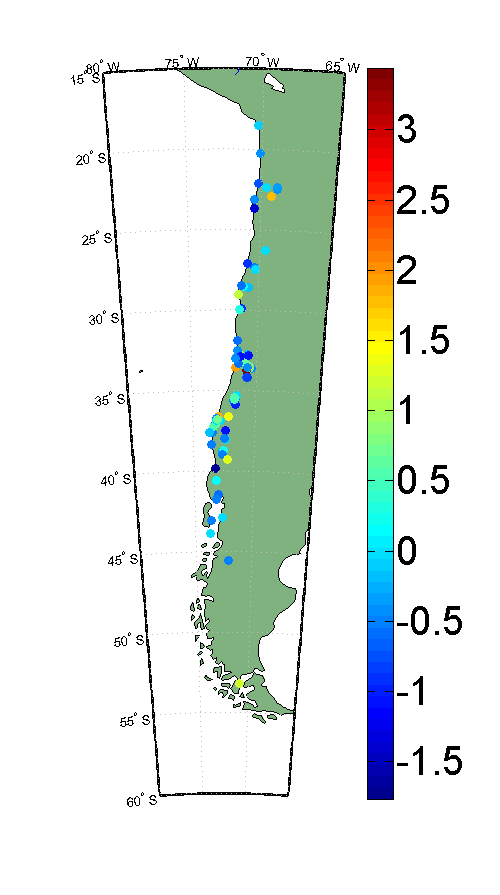
\includegraphics[width=0.7in,height=0.8in] {figures/Chile_absent_zscore_3.png}
		\label{fig:absent_Chile_score}
	}
	\hfill
	\subfigure[]{
		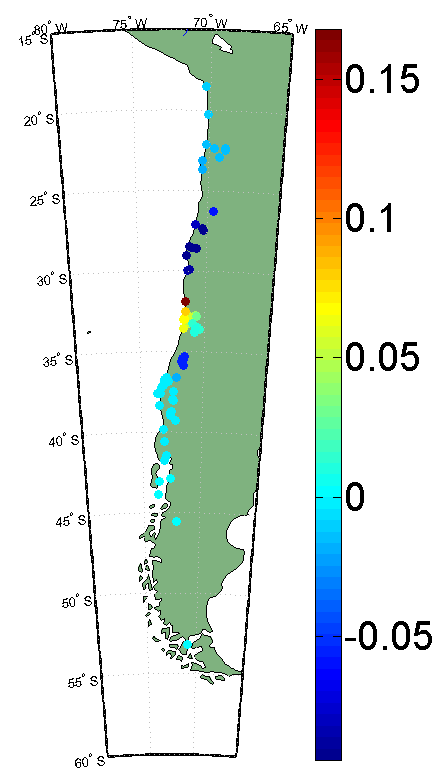
\includegraphics[width=0.7in,height=0.8in] {figures/Chile_absent_wavelet_3.png}
		\label{fig:absent_Chile_wavelet}
	}
	\hfill
	\subfigure[]{
		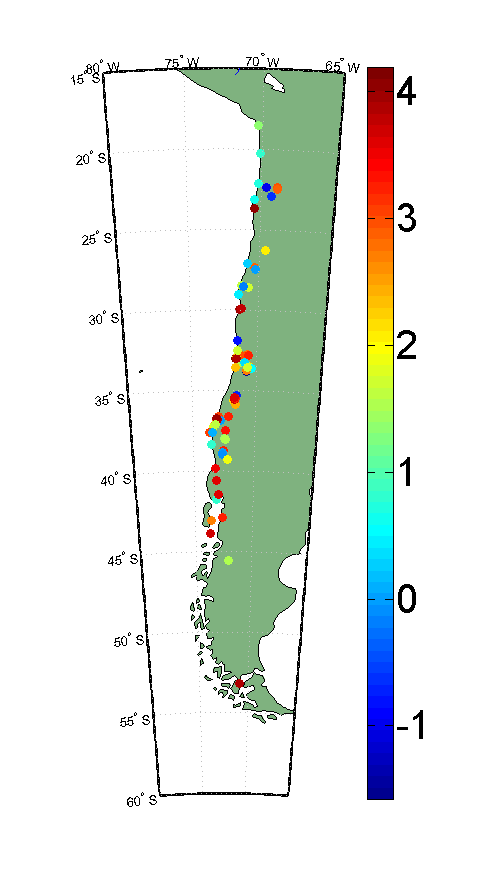
\includegraphics[width=0.7in,height=0.8in] {figures/Chile_burst_zscore_3.png}
		\label{fig:burst_Chile_score}
	}
	\hfill
	\subfigure[]{
		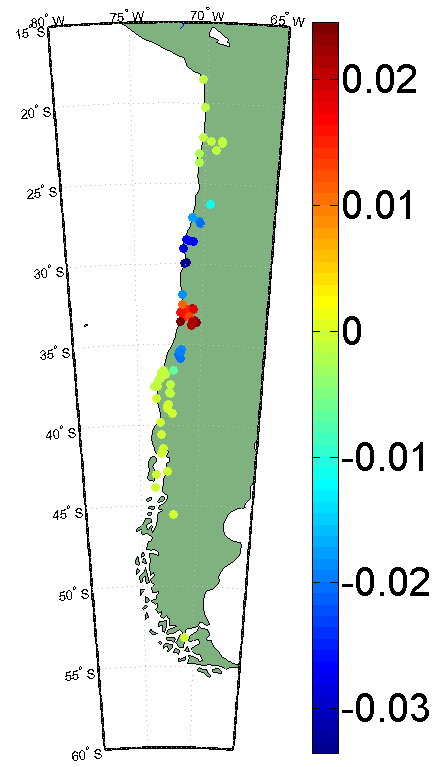
\includegraphics[width=0.7in,height=0.8in] {figures/Chile_burst_wavelet_3.png}
		\label{fig:burst_Chile_wavelet}
	}
	\subfigure[]{
		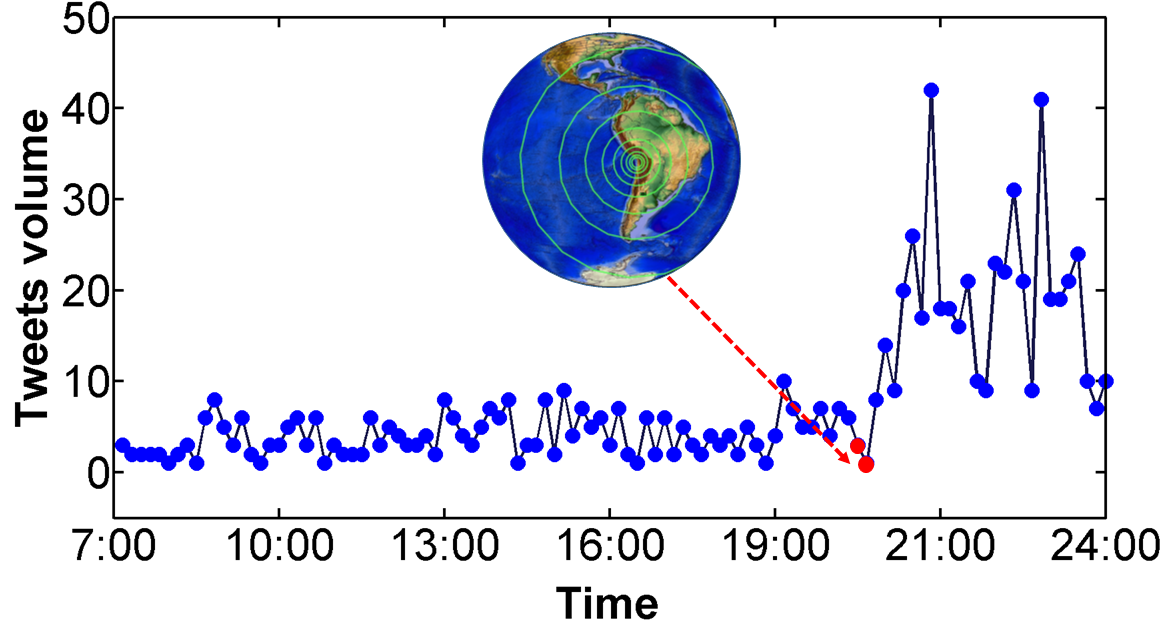
\includegraphics[width=1.4in,height=0.7in] {figures/earthquake_example_10min_circle.png}
		\label{fig:earthquake}
	}
	\subfigure[]{
		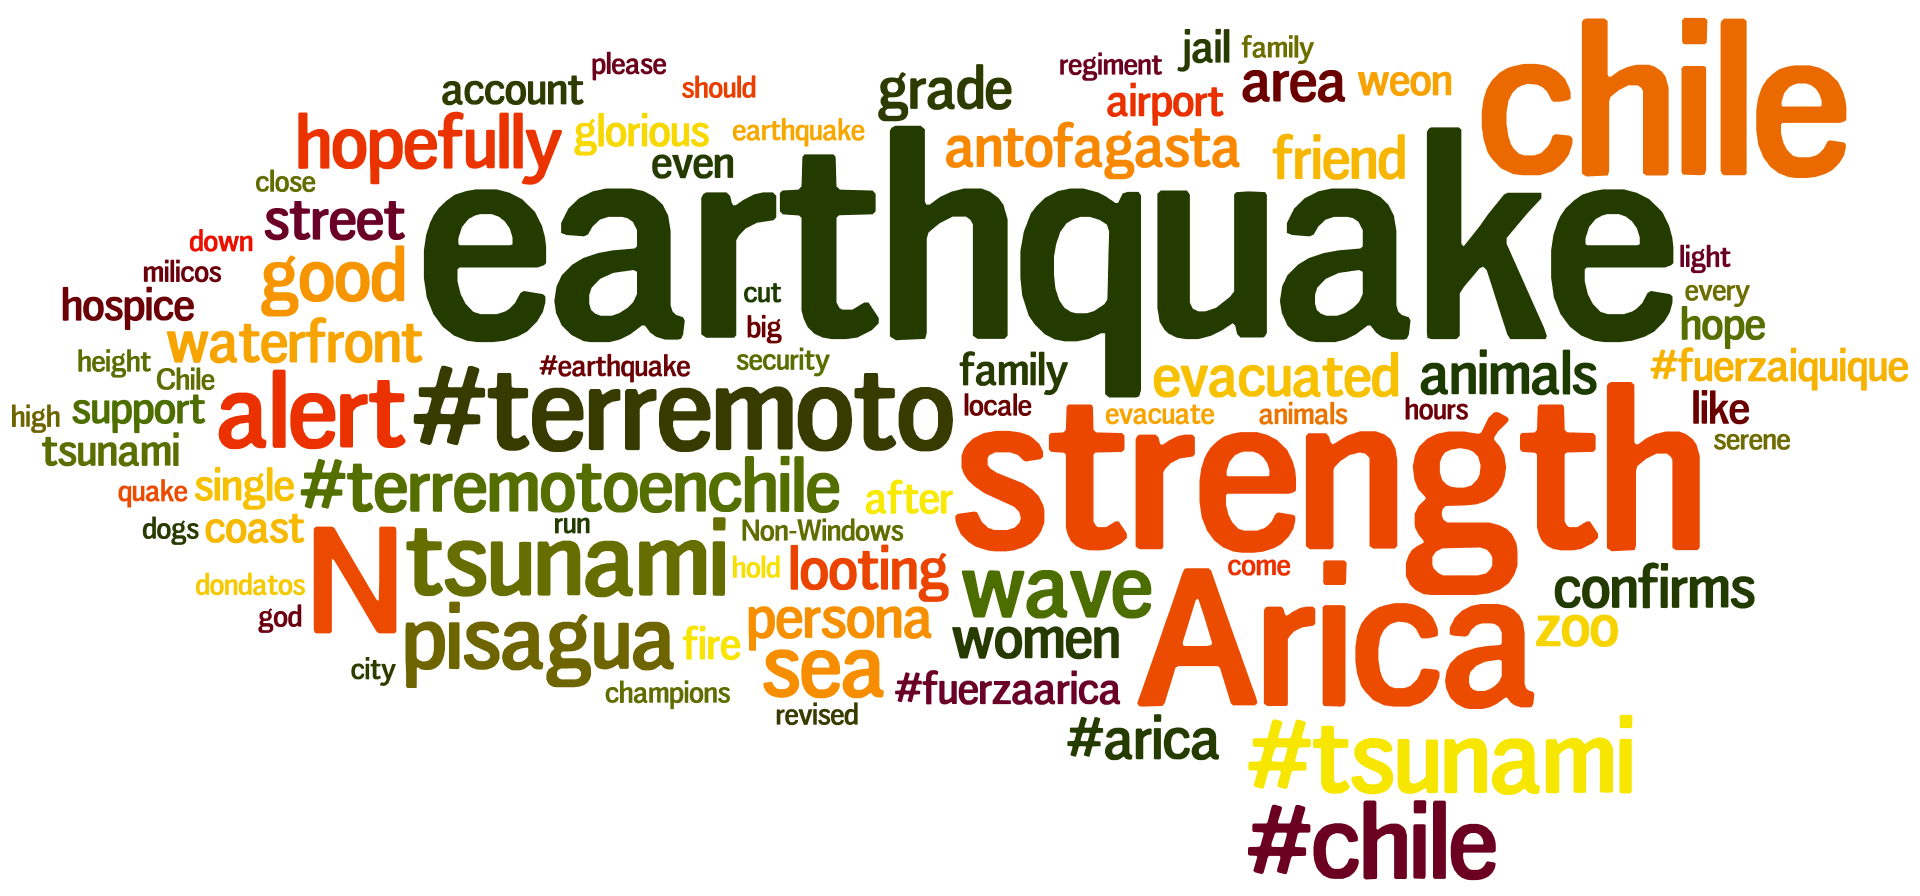
\includegraphics[width=1.4in,height=0.7in] {figures/earthquake_cloud.png}
		\label{fig:earthquake-cloud}
	}
	\caption{Iquique Earthquake, Chile. (a-d) plots show differences in distributions of absenteeism score and wavelet coefficients calculated at 8:45 PM, April 1, 2014 (a-b) involving group absenteeism and later when burst in activity is captured at 11:00 AM, April 2, 2014 (c-d), respectively; (e) Tweet time series for Iquique on April 1, 2014; (f) Word cloud of Tweets which mention `Iquique'.}
\label{fig:case1_wavelet}
\end{figure}



\textbf{Case study 1: Iquique Earthquake, Chile.}
On April 1, 2014 around 8:46 PM (local time) a large earthquake struck off the coast of Chile, northwest of the port city of Iquique.
We show the distribution of absenteeism scores and normalized wavelet coefficient values of the graph wavelets from the beginning of this event and over a 24 hour period.
As shown in Figure~\ref{fig:absent_Chile_score} we observe an absenteeism behavior, where the scores are dominated by very low (blue spectrum) of Z-score values (indicating high absenteeism).
Likewise in Figure~\ref{fig:absent_Chile_wavelet}, we witness low coefficients values for the northern regions of Chile, where the impact of the earthquake was most significant.
As the news of earthquake spread throughout the next day, user activity on social media increased. This bursty behavior is seen on April 2nd, around 11:00 AM. We can observe from Figure~\ref{fig:burst_Chile_score} that our Z-scores have increased (red spectrum) significantly and the coefficient value distribution (see Figure~\ref{fig:burst_Chile_wavelet}) of graph wavelets, for northern regions of Chile is now in red spectrum.
From the graph wavelet distributions in Figures~\ref{fig:absent_Chile_wavelet}~\ref{fig:burst_Chile_wavelet}, we can see that the kernel area of the absenteeism/burst wavelets cover most large negative/positive values.
In this way, the wavelet identifies the abnormal negative/positive groups in absent/burst time intervals, respectively.
Furthermore, a high correlation score of 0.726 was calculated for the wavelets from absenteeism and bursty periods of this episode.
As a result, we note that there is a strong connection between the burst in activity and the previously observed absenteeism, signaling an event was detected.




\begin{figure}[t]
	\centering
	\subfigure[]{
		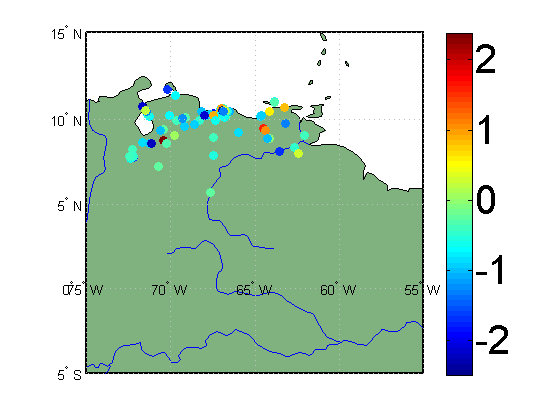
\includegraphics[width=0.7in, height=0.85in] {figures/Venuze_absent_zscore_3.png}
		\label{fig:absent_Venezuela_score}
	}
	\subfigure[]{
		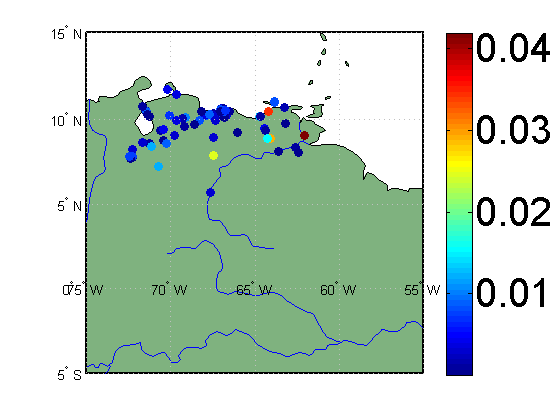
\includegraphics[width=0.7in,height=0.85in] {figures/Venuze_absent_wavelet_3.png}
		\label{fig:absent_Venezuela_wavelet}
	}
	\subfigure[]{
		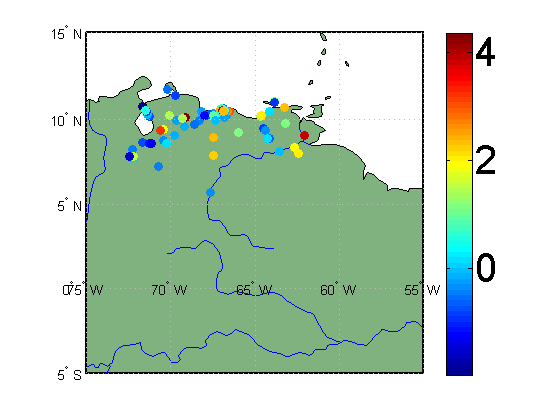
\includegraphics[width=0.7in,height=0.85in] {figures/Venuze_burst_zscore_3.png}
		\label{fig:burst_Venezuela_score}
	}
	\subfigure[]{
		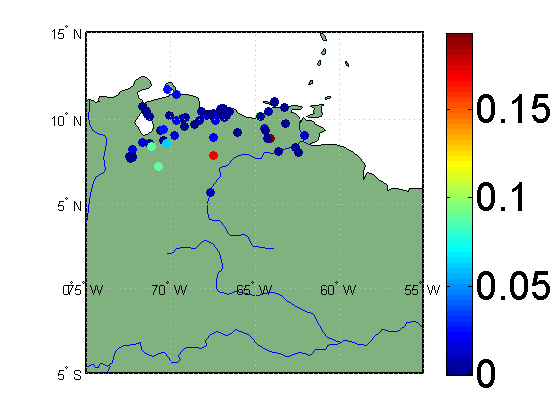
\includegraphics[width=0.7in,height=0.85in] {figures/Venuze_burst_wavelet_3.png}
		\label{fig:burst_Venezuela_wavelet}
	}
	\subfigure[]{
		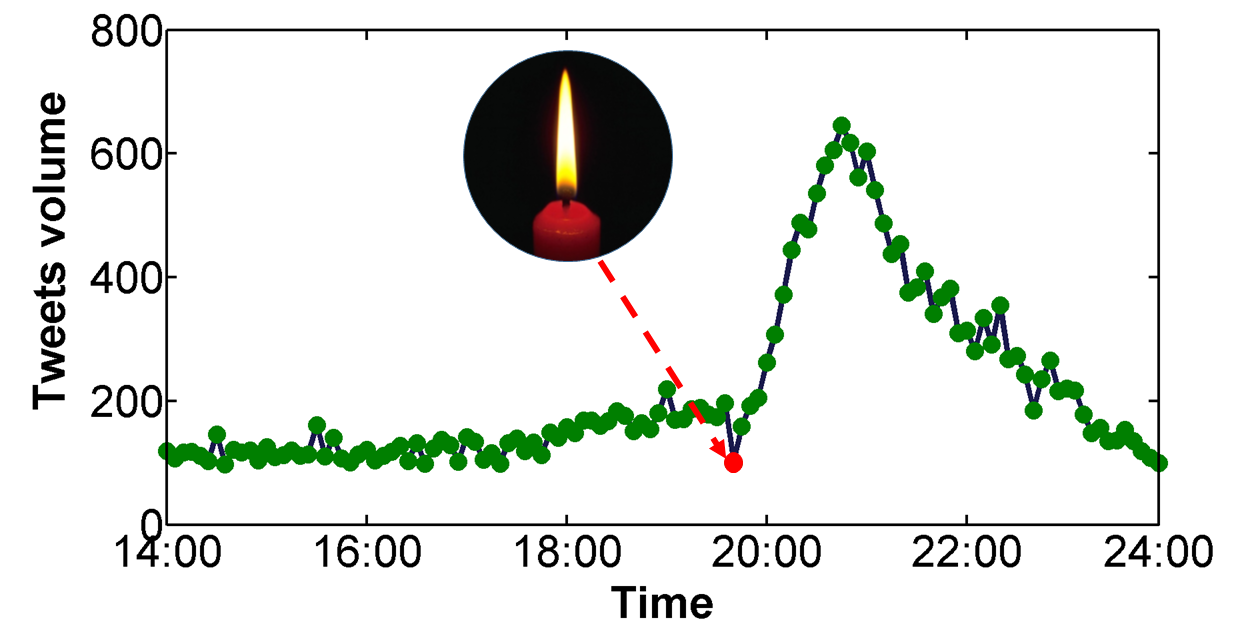
\includegraphics[width=1.4in,height=0.7in] {figures/Veneuela_power_count_all.png}
		\label{fig:power}
	}
	\subfigure[]{
		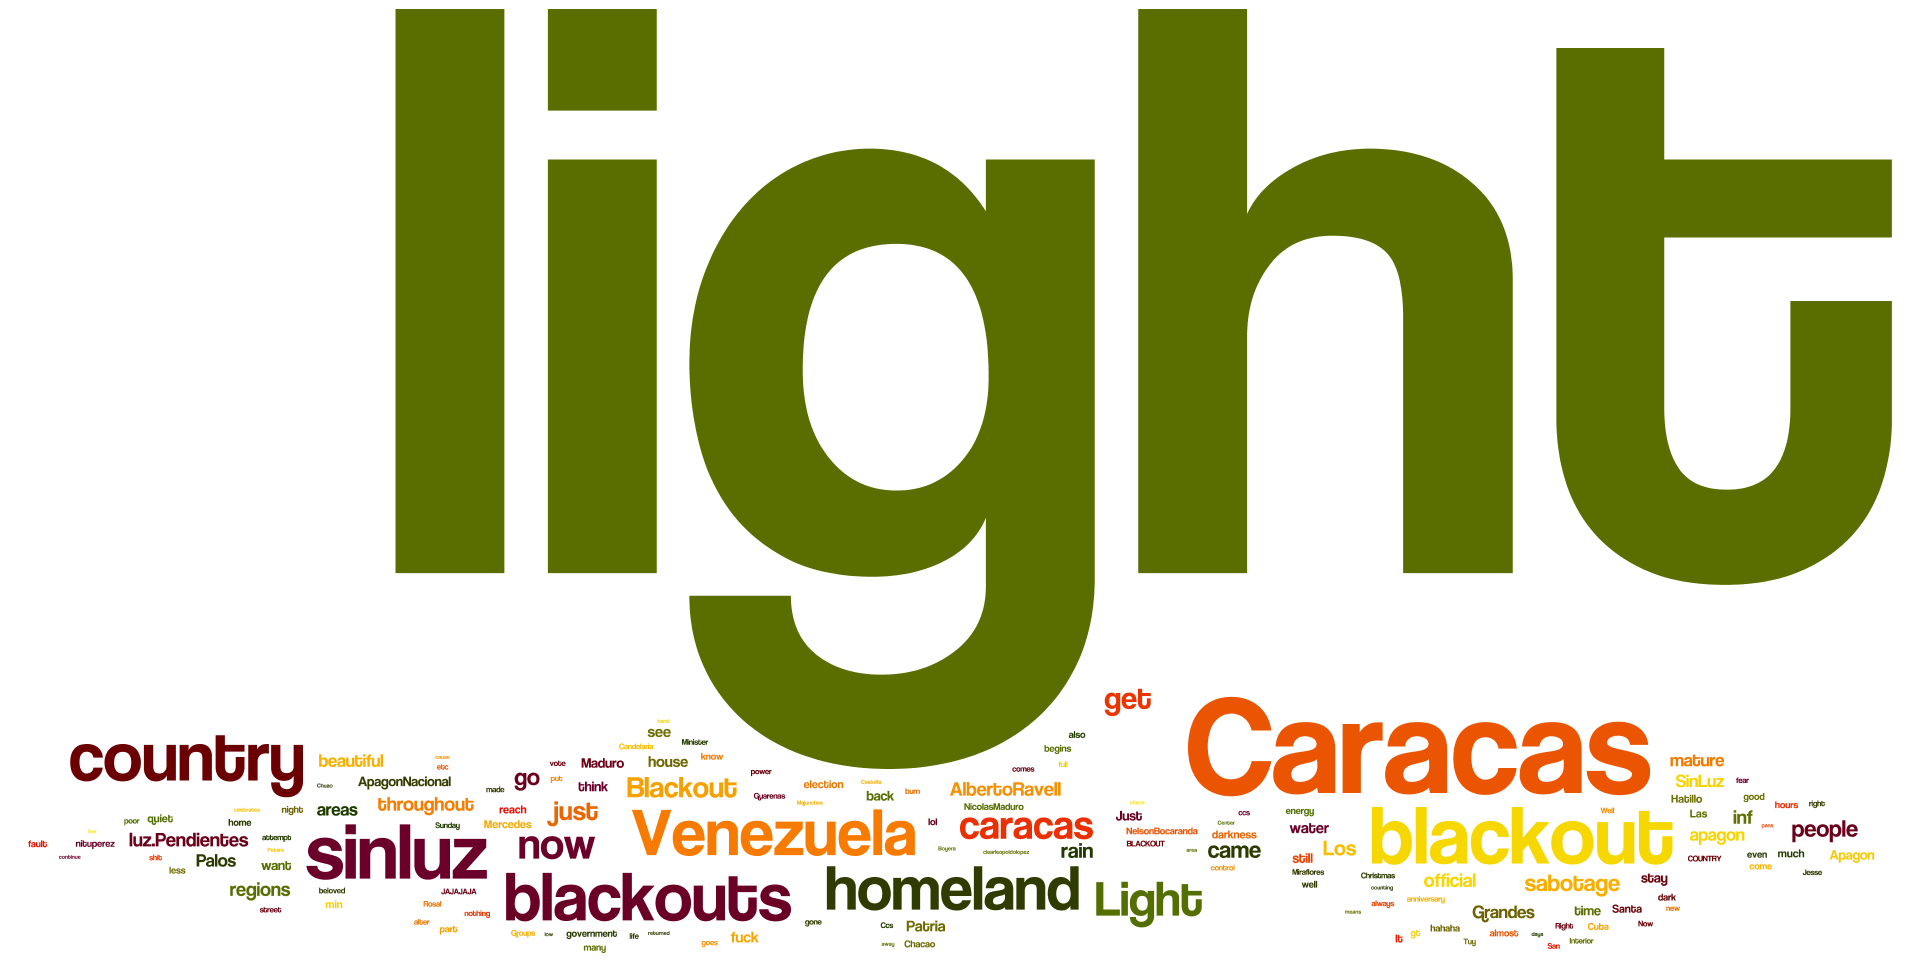
\includegraphics[width=1.4in,height=0.7in] {figures/power-English.png}
		\label{fig:power-cloud}
	}
	\caption{Power Outage in Venezuela. (a-d) plots show differences in distributions of absenteeism score and wavelet coefficients calculated at 7:40 PM, December 2, 2013 (a-b) involving group absenteeism and later when burst in activity is captured at 8:45 PM in the same day (c-d), respectively; (e) Time series of Tweets volume on December 2, 2013; (f) Word cloud of Tweets mentioning `Caracas'.}
\label{fig:case2_wavelet}
\end{figure}


From the graph wavelets generated in absenteeism time period Figure~\ref{fig:absent_Chile_wavelet}, we found the central node to be the city of `Iquique'.
We study the time series (Figure~\ref{fig:earthquake}) of Twitter activity for Iquique and word clouds (see Figure~\ref{fig:earthquake-cloud}) generated from their content, to see how events unfolded during the course of the earthquake.
Strong absenteeism is observed from 8:45 PM to 9:20 PM. We also checked  user mobility through geotagged Tweets from city of Iquique, on April 1, 2014 and found that the user mobility fraction had increased by 15.4\%.



\textbf{Case Study 2: Massive power outage in Venezuela.}
A massive power outage in Venezuela plunged several major cities including the capital city, Caracas in to darkness around 7:40 PM (local time) on December 2, 2013.
News media reported\footnote{http://www.usatoday.com/story/news/world/2013/12/\hskip0ex 02/\hskip0ex power-failure-caracas-venezuela/3823327/}, that the power outage lasted for 10-15 minutes, and the people of Caracas soon went out in the streets to protest.
This action at the beginning of the episode coincides with the absenteeism period detected by our algorithm.
The scatter plots showing distribution of absenteeism scores and wavelet coefficients (Figures~\ref{fig:absent_Venezuela_score},~\ref{fig:absent_Venezuela_wavelet}) indicate that most of the low values are less than $0$.
Shortly after the absenteeism, we detected a huge burst in activity around 8:45 PM, signaled by the increased z-scores (low absenteeism) and coefficient values (Figures~\ref{fig:burst_Venezuela_score},~\ref{fig:burst_Venezuela_wavelet}).
A correlation score of 0.617 was calculated on comparing the graph wavelets from both absentee and burst period.

The absenteeism related graph wavelets indicated that the city of Caracas
%`San Fernando de Apure'
was the central node. Taking a close look at the Twitter volume and Tweets from Caracas and surrounding cities, we observed a sharp decline in user activity right around 7:40 PM and then a huge spike starting at 8:45 PM.
The word clouds of Tweet content show a very similar story.
The most dominant words are `light' and `blackout', even the Spanish phrase `sin luz' which means `no light' became a trending hashtag \#sinluz on Twitter.



\begin{figure}[t]
	\centering
	\subfigure[]{
		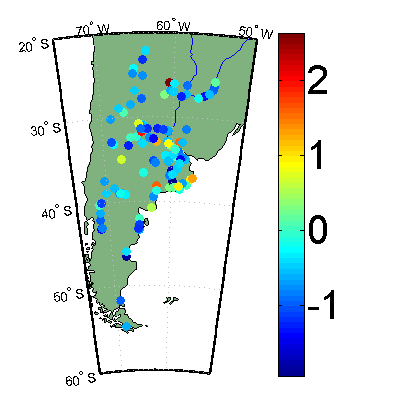
\includegraphics[height=0.9in] {figures/Argentina_absent_zscore_3.png}
		\label{fig:absent_Argentina_score}
	}
	\subfigure[]{
		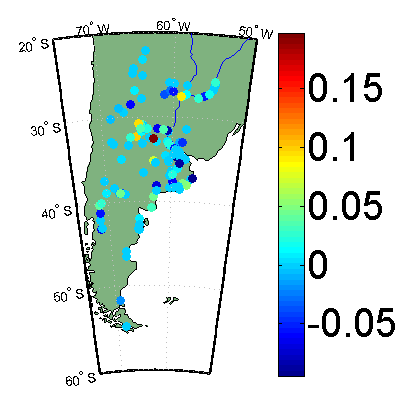
\includegraphics[height=0.9in] {figures/Argentina_absent_wavelet_3.png}
		\label{fig:absent_Argentina_wavelet}
	}
	\subfigure[]{
		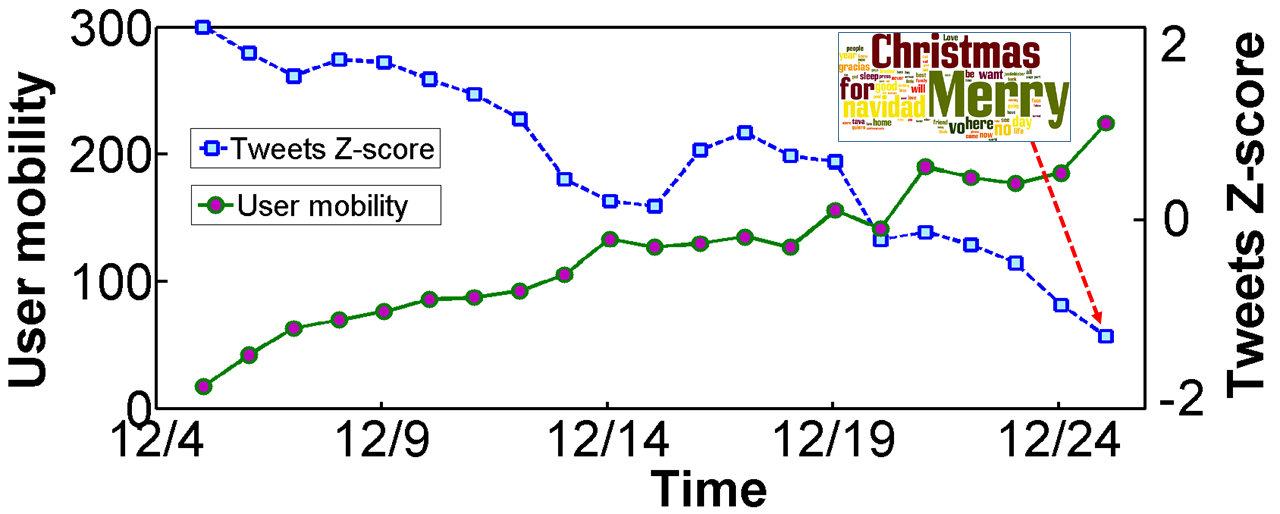
\includegraphics[width=1.3in, height=0.7in] {figures/holiday-cloud.png}
		\label{fig:holiday-cloud}
	}
	\caption{The Christmas Day in Argentina: (a-b) plots show distributions of (a) absenteeism score and (b) wavelet coefficients calculated on December 25, 2013; (c) Time series comparing absenteeism score and user mobility corresponding to Tweets between December 5 - 25, 2013.}
\label{fig:case3_wavelet}
\end{figure}


\textbf{Case Study 3: Christmas Day.}
As mentioned earlier, an absenteeism behavior may not always lead to a spike in activity. In this case, our model detected strong absenteeism in social media activity for major holidays such as Christmas day, however it was not followed by a bursty period in Twitter activity. One explanation of this behavior is that people tend to travel back to visit family during the holidays. This is supported by low values of Z-scores or high absenteeism in Figure~\ref{fig:absent_Argentina_score} and wavelet coefficients in Figure~\ref{fig:absent_Argentina_wavelet} with respect to Argentina Tweets on December 25, 2013. Hence, no subsequent burst period was detected for this event. Interestingly, as the Christmas day approached we observed (see Figure~\ref{fig:holiday-cloud}) that user mobility gradually increases and Z-score decreases signaling greater absenteeism. We used Pearson's correlation coefficient to measure the two time series and found a correlation score of -0.94.

\subsection{Why Absenteeism Group Detection?}
Previous research has demonstrated the importance of burst detection in Twitter. In our study, we argue that group absenteeism can also be vital for detecting disruptive societal events. Modeling absenteeism is crucial, because it can serve as a surrogate signal for event detection. For example, in the case of the Iquique earthquake, where our algorithm  detected an absenteeism behavior on Twitter followed by a spike in user activity. Unlike traditional event detection methods which identify real time events only after they have occurred i.e., once the burst signal has been identified; the absenteeism signal can be observed much earlier, and it renders a foresight or view into the future events. Our approach thus offers a significant advantage over current strategies that focus solely on modeling spike or burst related patterns for event detection.

%Disruptive events which cause Twitter absenteeism, but also render burst detection methods less useful. In the case of the Natal protest event, a large portion of people were walking on the street to protest, and the city's tweet absenteeism score reached a minimum. During the Brazil floods, the tweets tended to become inactive as the severity of the floods increased. It reached the lowest point when the flood was at its worst. In these two cases in particular, using a burst signal alone it can be difficult to identify such events.

\section{Conclusion}
\label{sec:conclusion}
Existing approaches for event detection suffer from an inherent latency in their detection process. It is because they use the bursty signals from abnormal activity on social networks, but miss the absenteeism signal that precedes these bursts. Our approach bridges this shortcoming by successfully modeling this \textit{lull-ness}. We defined an absenteeism score over the groups of cities that form our Twitter network and used it to construct wavelet transforms, that not only to detect the anomalous subgraphs (including both burst and absenteeism groups) at different scales, but also to find the geographical focal point of the anomaly. What is more, the localization property of graph wavelet guarantees the selected groups to be automatically compact. Those identified abnormal groups are verified and proved to be indicative at detecting events such as man-made protests or natural disasters.
%In this work, we have presented a systematic and unified framework for detecting, identifying event's location and distinguishing anomalous groups in Twitter.

%From the three case studies, we have shown that the initial phase in the evolution of a disruptive, event is characterized by group absenteeism behavior. This behavior is further underlined by an increase in user mobility. As in the case of ``Christmas Day" event we observed absenteeism from Argentina Twitter users in days leading to December 25th was characterized by increased mobility (inferred from geolocated tweets).

%In future work, we plan to extend our detection model to capture extent of an event's influence over network. Another interesting extension of our work would be to include absenteeism as feature to classify event of different nature (disruptive vs non-disruptive).

%Graph wavelet based approach, considering both the graph structure and the vector f;
%Define an anomaly index of f�s distribution on G;
%Identify abnormal locations using graph wavelet;
%Detect absent and burst groups simultaneously.

%\section*{Acknowledgment}
%
%
%The authors would like to thank...


%%%%%%%%%%%%%%%%%%%%%%%%%%%% end %%%%%%%%%%%%%%%%%%%%%%%%%
%\begin{table*}[th] %!htp
% \renewcommand{\arraystretch}{1}
% \caption{\label{table:list_events} Selected major events in South America countries}
% \scriptsize
% \centering
% \begin{tabular}{ p{0.5cm}| p{2cm} | p{2.2cm} | p{2.2cm} | p{2.2cm} | p{2.5cm} | p{3cm} }
%  \hline
%  \textbf{No.} & \textbf{Events}& \textbf{ Absenteeism } & \textbf{Response time} & \textbf{Correlation}&\textbf{Central location} \\ [1ex]
%  \hline
%        1& Earthquake & 8:45 PM & 3 hours & 0.73 &Iquique, Chile\\
%        2& Blackout & 7:40 PM & 1 hour & 0.81& Caracas, Venezuela \\
%        3& holiday & one day & 2 days & 0.33 & \\        \hline
% \end{tabular}
%\end{table*}


%Public holidays are typical events causing group absenteeism. One of the most dominant reason is, during public holidays, especially long-time holiday, people tend to travel, which resulting in a high level of local user mobility, and users' mobility will cause Twitter absenteeism accordingly.
%We calculating more cases Pearson's correlation, and plot their distribution in Figure~\ref{fig:pearson}, of which the median value of correlation score is -0.88, and the average correlation score is -0.79. We can see the user mobility plays a forceful role in influencing Twitter absenteeism.

%\subsection{Performance}
%We use the data set on February 27, 2014, and set the time window as one day. We plot the comparison results from two aspects:  running time complexity, and parameter sensibility in figure~\ref{fig:performance},~\ref{fig:running_time},~\ref{fig:sensibility}.
%\begin{figure}[ht]
%	\centering
%	\subfigure[matrix]{
%		\includegraphics[width=1.55in,height=1in] {figures/performance1.png}
%		\label{fig:performance1}
%	}
%	\subfigure[graph]{
%		\includegraphics[width=1.55in,height=1in] {figures/performance2.png}
%		\label{fig:performance2}
%	}
%	\caption{running time vs input parameter.}
%	\label{fig:performance}
%\end{figure}
%\paragraph{Running time}From Figure~\ref{fig:performance}, we can see that the running time of minimal matrix approach increases extremely fast when $A$ is larger than 0.09. While in graph wavelet approach, the increasing speed is much stable as $d_{th}$ increases. This is because minimal matrix approach's time complexity is in proportion to $A^2$, while graph wavelet approach's time complexity is proportional to $d_{th}$. From Figure~\ref{fig:running_time}, we can see clearly that for the minimal matrix algorithm, the running time complexity also increase sharply with the input size $n$, while in graph wavelet approach, the increase speed is moderate. This is because the minimal matrix approach's timing complexity is $O(N^3)$, while graph wavelet approach's time complexity is $O(N^2)$. Thus, the graph wavelet approach is better  than minimal matrix approach in term of running time for a larger absenteeism group.
%\begin{figure}[h]
%	\centering
%	\subfigure[matrix]{
%		\includegraphics[width=1.55in,height=1in] {figures/running_time1.png}
%		\label{fig:running1}
%	}
%	\subfigure[graph]{
%		\includegraphics[width=1.55in,height=1in] {figures/running_time2.png}
%		\label{fig:running2}
%	}
%	\caption{Running time vs input size.}
%	\label{fig:running_time}
%\end{figure}
%\paragraph{Parameter sensibility}In minimal matrix approach, set the input parameter as $A$, and the optimal absenteeism group as $P_{min}$. When $A$ is changed to $A$', the optimal absenteeism group is changed to $P_{min}$, define the output error as the city number that exists in $P_{min}$ but not in $P_{min}'$, and denoted as $P_{min}-P_{min}'$. We define the parameter sensibility as: $$sensibility=\frac{{|P_{min}-P_{min}'|}/{|P_{min}|}}{|A-A'|/{A}}.$$ We plot the minimal matrix approach and graph wavelet approach's sensibility in Figure~\ref{fig:sensibility}. In the minimal matrix approach, when the input parameter error is smaller than 20\%, the output absenteeism group error is less than 5\%. While in the graph wavelet approach, the output absenteeism group error is linear to the input error parameter. This is probably because minimal matrix approach aggregates all the absenteeism score covered by the region, and usually has a much larger city number than the graph wavelet approach, and makes minimal matrix approach better at anti-noise.  All in all, the minimal matrix algorithm focuses on all the cities in the cover group, and has a better global performance at anti-noise, while is inferior to the graph wavelet counterpart in term of running time complexity.
%\begin{figure}[h]
%	\centering
%	\subfigure[matrix]{
%		\includegraphics[width=1.55in,height=1in] {figures/sensibility1.png}
%		\label{fig:sensibility1}
%	}
%	\subfigure[graph]{
%		\includegraphics[width=1.55in,height=1in] {figures/sensibility2.png}
%		\label{fig:sensibility2}
%	}
%	\caption{Sensibility comparison of the two algorithms.}
%	\label{fig:sensibility}
%\end{figure}




% % % % % % % % % % % % % the end% % % % % % % %
%
%\begin{figure}[ht]
%	\centering
%	\subfigure[]{
%		\includegraphics[width=1.55in,height=1in] {figures/Curitiba-Brazil1-cloud.png}
%		\label{fig:holiday}
%	}
%	\subfigure[]{
%		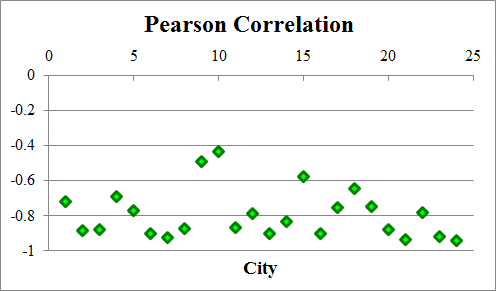
\includegraphics[width=1.55in,height=1in] {figures/pearson1.png}
%		\label{fig:pearson}
%	}
%	\caption{(a) User mobility time series and corresponding absenteeism score, from Dec 5, 2013 to Dec 25, 2013. (b) Pearson correlation score distribution of user mobility and absenteeism score.}
%\label{fig:case3}
%\end{figure}

%Now we show experimental results of our algorithm on highlighted case studies (see Table~\ref{table:list_events}):
%
%\begin{table*}[th] %!htp
%	\renewcommand{\arraystretch}{1}
%	\caption{\label{table:list_events} Selected major events in South America countries}
%	\scriptsize
%	\centering
%	\begin{tabular}{ p{0.5cm}| p{1.5cm} | p{8cm} | p{1.5cm}}
%		\hline
%		\textbf{No.} & \textbf{Date}& \textbf{ Events} & \textbf{Test Areas}   \\ [1ex]
%		\hline
%        1& 2013-06-17 & Brazilian Spring: Protests in over 100 cities, over 2 million people & Brazil  \\		
%        2& 2013-12-02 & Power cut leaves much of Venezuela without electricity & Venezuela \\
%        3& 2013-12-24 & Floods, more than 50,000 people are forced to flee their homes & Brazil\\
%        4& 2013-12-25 & Christmas holiday  & Argentina \\
%        5& 2013-12-30 & Power supply disrupted in heatwave in Buenos Aires, Argentina & Argentina \\
%        6& 2014-04-01 &  M8.2 earthquake struck off the coast of Chile, epicenter is Iquique & Chile  \\
%        7 & 2014-05-21 & Bus strike paralyzes Brazil's biggest city as World Cup looms & Brazil \\			\hline
%	\end{tabular}
%\end{table*}


%The wavelet scales $t_j$ are selected to be logarithmically equispaced between the minimum and maximum scales $t_J$ and $t_1$, with the upper bound $\lambda_{max}$ of the spectrum of $L$. The placement of the maximum scales $t_1$ as well as the scaling function kernel $h$ will be determined by the selection of $\lambda_{min}=\frac{\lambda_{min}}{K}$, where $K$ is a design parameter of the transformation. We then set $t_1$ so that $g(t_1x)$ has power-law decay for $x>\lambda_{min}$, and set $t_J$ so that $g(t_Jx)$ provides monotonicity of the polynomial for $x < \lambda_{max}$. This is achieved by $t_1=\frac{x_2}{\lambda_{min}}$, and $t_J=\frac{x_2}{\lambda_{max}}$. For the scaling function kernel we take $h(x)=\gamma exp(-({{\frac{x}{\lambda_{min}}}})^4)$, where $\gamma$ is set such that $h(0)$ has the same value as the maximum value of $g$.
%
%At each time point the graph has an Z-score vector $f$ and when we get the lowest value for function $< \psi_{t,n},f>$ the corresponding wavelet $\psi_{t,n}$ is reported as an absenteeism pattern.






%\paragraph{\textbf{Event Impact}}
%The absenteeism event impact is defined as:
%\begin{equation}
%AEI = (|W'_f(t_l,n_l;l)|+1)*|W'_f(t_\tau,n_\tau;\tau)|*\frac{t_\tau}{t_l}.
%\end{equation}
%\paragraph{\textbf{Response Time}} The absenteeism event response time is defined as:
%\begin{equation}
% t_{rsp}= \tau-l.
%\end{equation}



% conference papers do not normally have an appendix


% use section* for acknowledgment





% trigger a \newpage just before the given reference
% number - used to balance the columns on the last page
% adjust value as needed - may need to be readjusted if
% the document is modified later
%\IEEEtriggeratref{8}
% The "triggered" command can be changed if desired:
%\IEEEtriggercmd{\enlargethispage{-5in}}

% references section

% can use a bibliography generated by BibTeX as a .bbl file
% BibTeX documentation can be easily obtained at:
% http://mirror.ctan.org/biblio/bibtex/contrib/doc/
% The IEEEtran BibTeX style support page is at:
% http://www.michaelshell.org/tex/ieeetran/bibtex/
%\bibliographystyle{IEEEtran}
% argument is your BibTeX string definitions and bibliography database(s)
%\bibliography{IEEEabrv,../bib/paper}
%
% <OR> manually copy in the resultant .bbl file
% set second argument of \begin to the number of references
% (used to reserve space for the reference number labels box)
%\begin{thebibliography}{1}
%
%\bibitem{IEEEhowto:kopka}
%H.~Kopka and P.~W. Daly, \emph{A Guide to \LaTeX}, 3rd~ed.\hskip 1em plus
%  0.5em minus 0.4em\relax Harlow, England: Addison-Wesley, 1999.
%
%\end{thebibliography}


\bibliographystyle{IEEEtranS}
%\bibliographystyle{splncs03}
\bibliography{my-icdm}



% that's all folks
\end{document}



%
%\begin{figure}[h]
%	\centering
%    {
%		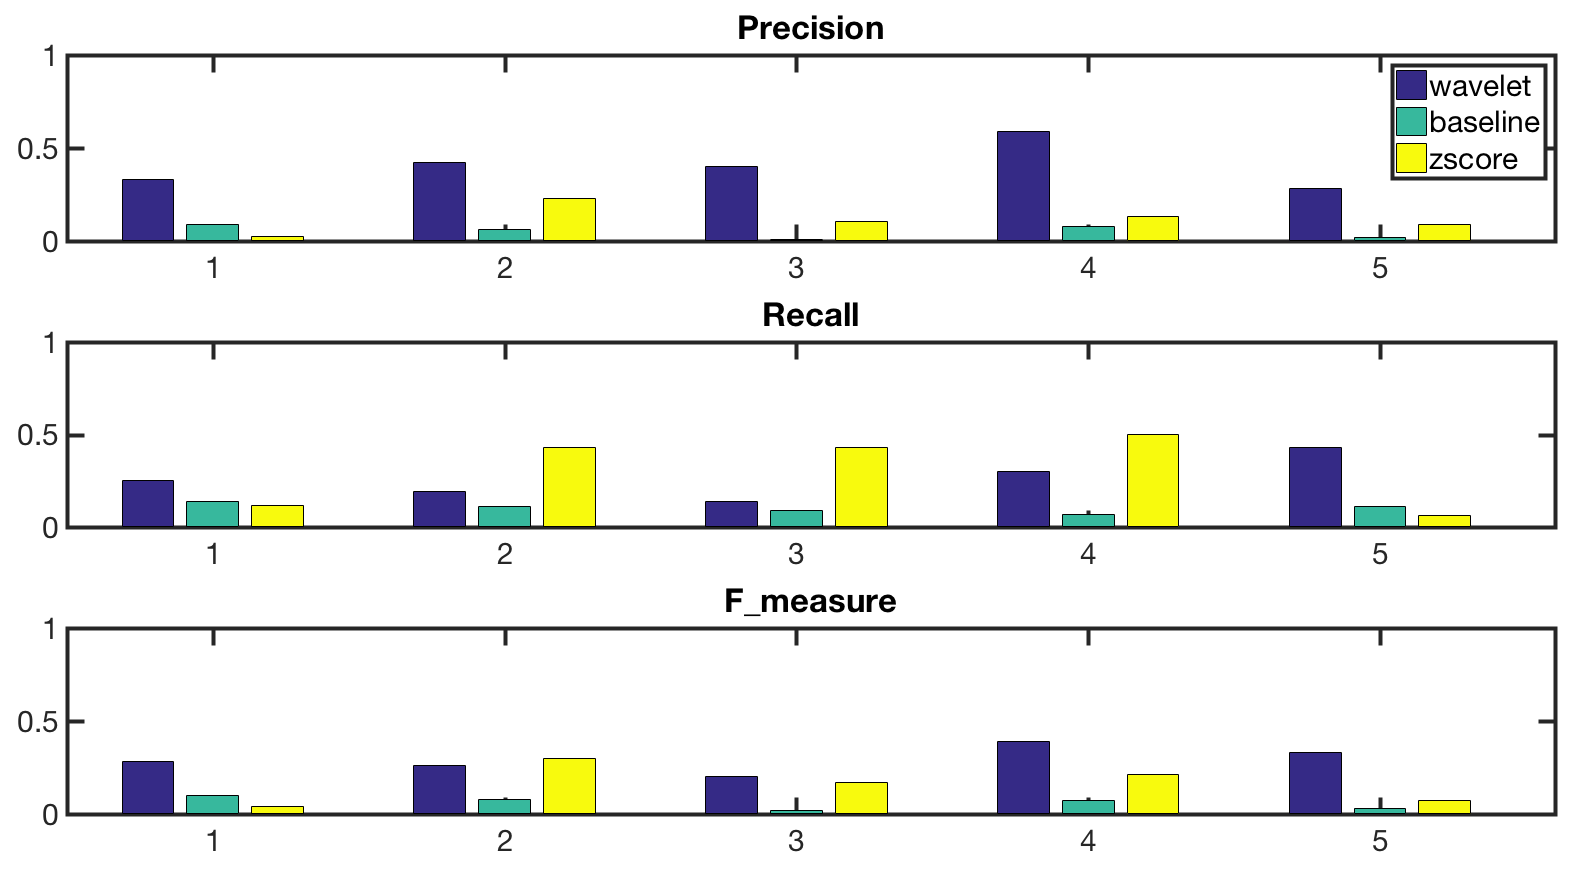
\includegraphics[width= 3in] {figures/performance_compare_bar_graph_brazil.png}
%		\label{fig:distribution2}
%	}
%	\caption{Brazil protest detection performance.}
%	\label{Brazil_performance}
%\end{figure}
%
%
%\begin{figure}[h]
%	\centering
%    {
%		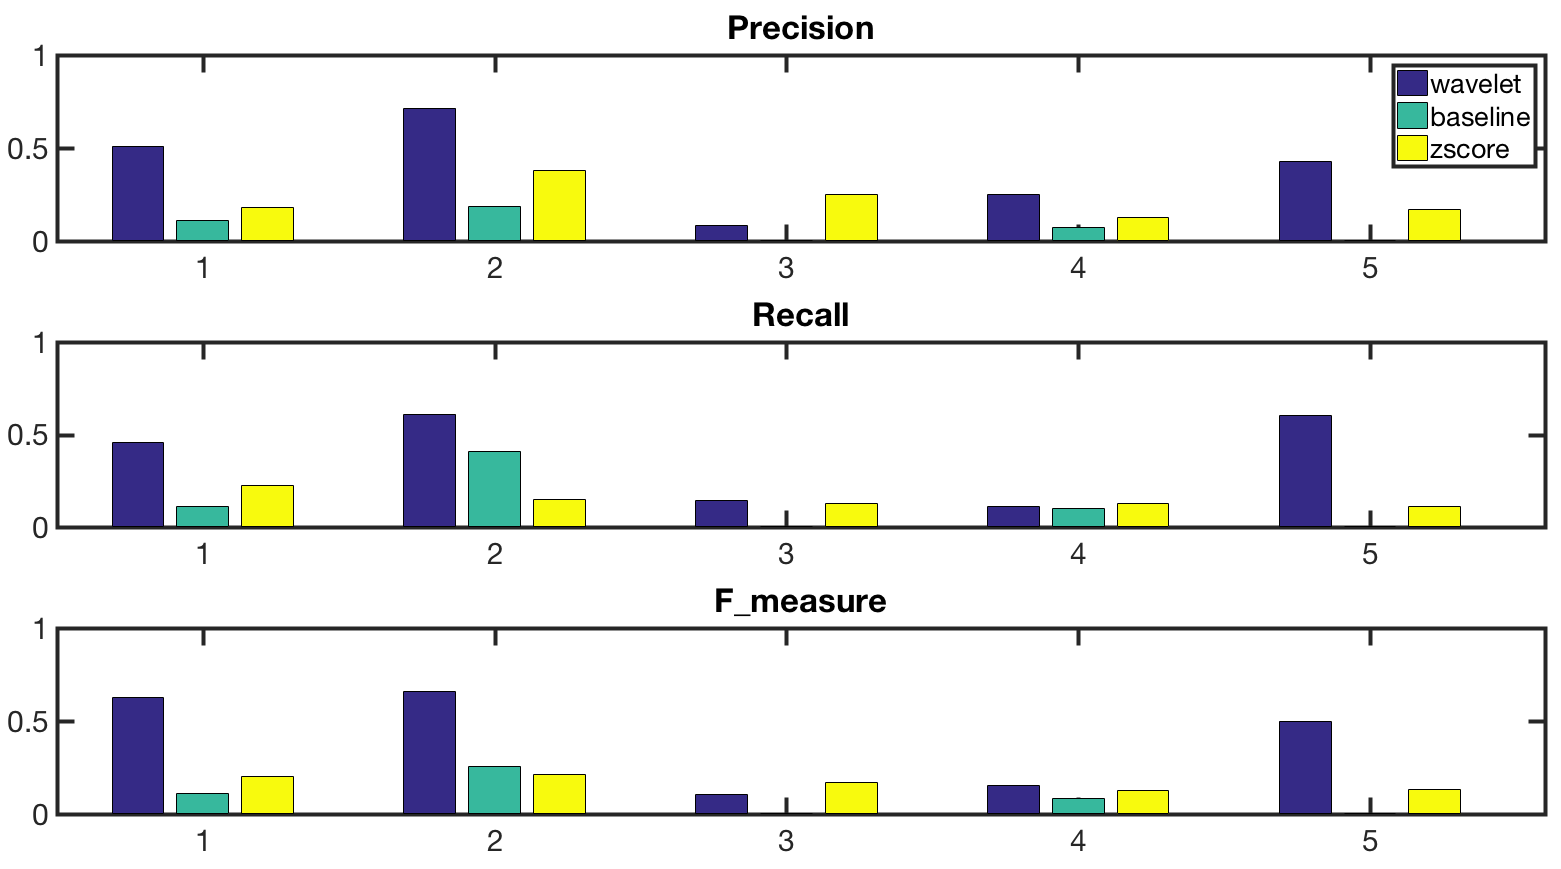
\includegraphics[width= 3in] {figures/performance_compare_bar_graph_mexico.png}
%		\label{fig:distribution2}
%	}
%	\caption{Mexico protest detection performance.}
%	\label{Mexico_performance}
%\end{figure}
%
%
%\begin{figure}[h]
%	\centering
%    {
%		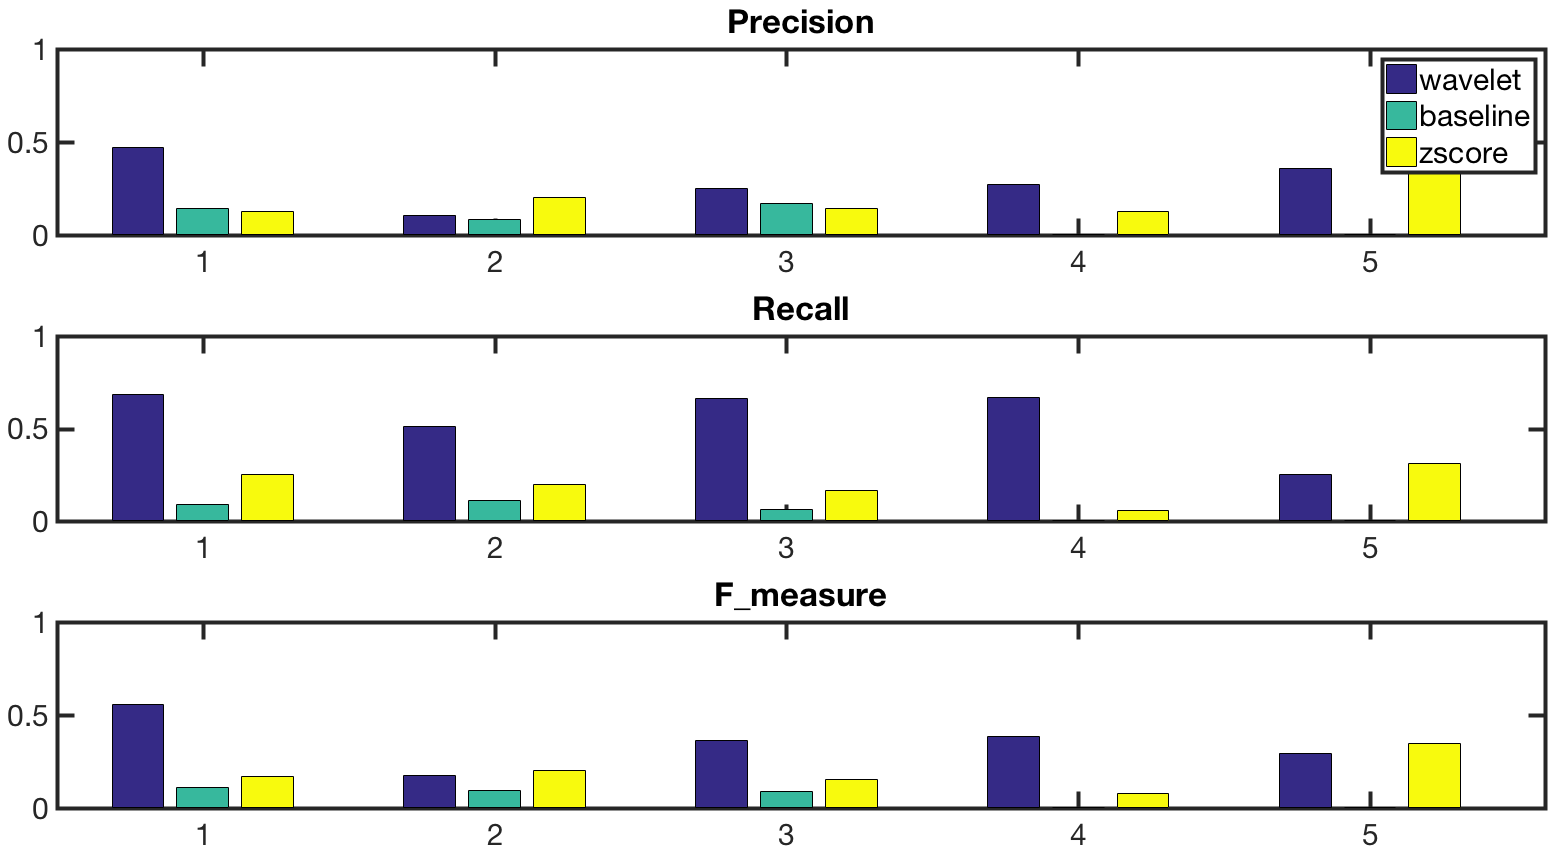
\includegraphics[width= 3in] {figures/performance_compare_bar_graph_venezuela.png}
%		\label{fig:distribution2}
%	}
%	\caption{Venezuela protest detection performance.}
%	\label{Venezuela_performance}
%\end{figure}






% {\textbf{Remarks:}} Essentially, the wavelet frame is generated by kernel function $g(x)$ and scaling function $h(x)$ with $J$ different scales. Those functions are also called filter banks. Figure~\ref{fig:brazil_filter} shows the wavelet filter banks for Brazil graph which we will mention in the experiment part.

% \begin{figure}[h]
% 	\centering
%     {
% 		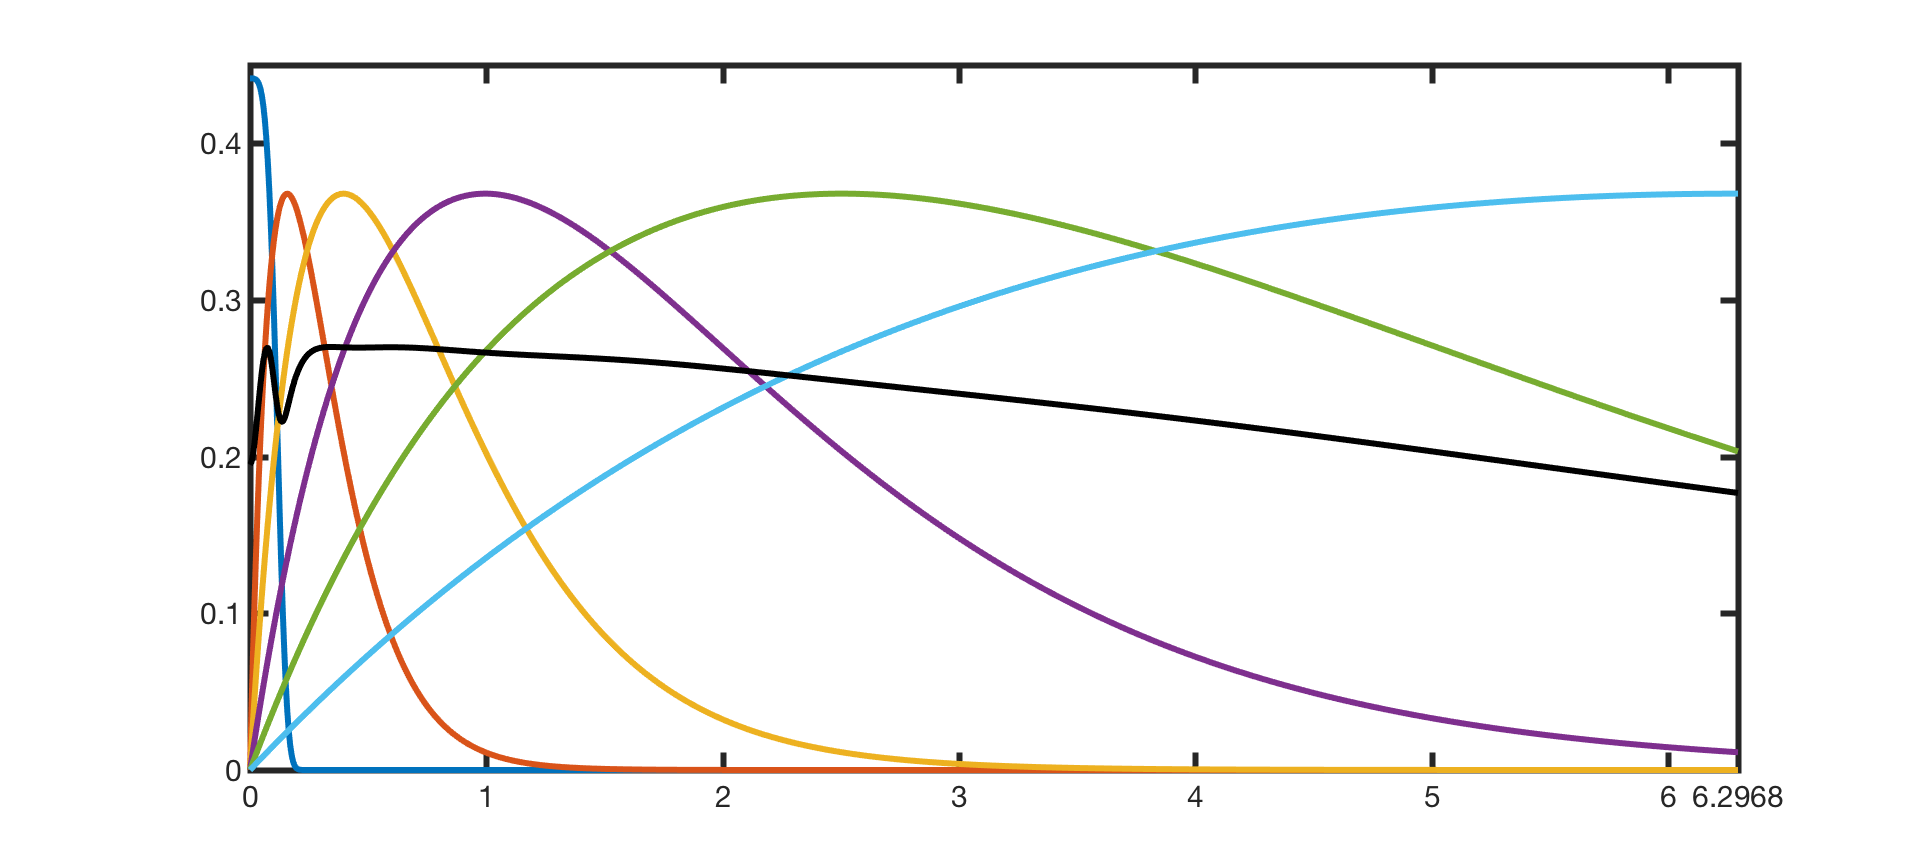
\includegraphics[width= 3.2in] {figures/brazil_filter.png}
% 		\label{fig:distribution2}
% 	}
% 	\caption{Wavelet filter banks for Brazil graph.}
% 	\label{fig:brazil_filter}
% \end{figure}



%\subsection{Group Absenteeism Event Detection}
%\label{sec:Group Absenteeism Event Detection}
%In our real world, there are various scenarios that causes people silent in social media for a certain amount of time. Take Earthquake emergence for example, when earthquake is happening, people hardly get a chance to use social media ( communication infrastructure might be paralyzed), thus it causes twitter volume in the affected area abnormal low. Some other examples, like flooding, blackout, and so on, often bring about similar phenomena. We call this kind of events as absenteeism event. When absenteeism event is over, and people's circumstance return to normal, it follows some kind of burst in social media since it's natural for people to talk about their experience concerning the absenteeism event. Usually, the severer of the absenteeism event is, the stronger absenteeism of the social media may present during the event, and the stronger burst will follow after.
%
%We propose a novel two-pass absenteeism based event detection algorithm. The underlying rationale of this algorithm is based on the following concepts.
%\begin{enumerate}
%\item At time interval $l$, using algorithm~\ref{algo:event_detection1} to identify absenteeism groups. For each absenteeism group $\mathcal{K}(s_j,a)$, it search burst groups $\mathcal{K}(s_k,b)$ which happens within a time window $L$. We claim that the time delay between $\mathcal{K}(s_j,a)$ and $\mathcal{K}(s_k,b)$ should be smaller than $L$, if the former is caused by the latter. When the time delay is larger that some pre-set $L$,  we claim that the burst group and the absenteeism group are uncorrelated.
%\item $\mathcal{K}(s_j,a)$ and $\mathcal{K}(s_k,a)$ should also be geographically correlated. This is because people are more likely to pay attention to events around where they live. To mathematically measure the geographically closeness of two city sets $\mathcal{K}(s_j,a)$ and $\mathcal{K'}(s_k,b)$, we define closeness $\rho(\mathcal{K}(a),\mathcal{K'}(b))$ as
%\begin{equation}
%\label{eq:eventsimilarity}
%\rho(\mathcal{K}(s_j,a),\mathcal{K'}(s_k,b)) = \frac{|\mathcal{K}(s_j,a)\cap\mathcal{K'}(s_k,b)|}{|\mathcal{K}(s_j,a)|\cdot|\mathcal{K'}(s_k,b)|}
%\end{equation}, where $|\mathcal{K}(\cdot)|$ is the city number. When $\rho$ is above some threshold $\rho_{th}$, we infer that an absenteeism event occurred and that it evolved on social networks into distinct phases: first group absenteeism, followed by a spike or burst in user activity. We denote this absenteeism event as e$\{\mathcal{K}(s_j,a),\mathcal{K}(s_k,b),\tau\}$, $\tau$ is the time delay.
%\item The computational complexity is $O(|\mathcal{I}^{bur}|\cdot |\mathcal{I}^{abs}|\cdot L\cdot |V|)$, and is $O(L|V|^3)$ in worst cases.
%%For instance, taking the power-cut-off for instance, usually only people who live in the affected area will ``yield at " this event a lot because it brings inconvenience to their life. However, people who live outside of the affected areas would hardly mention this event. Thus, to measure the correlation between absenteeism pattern and burst pattern is proposed as:
%\end{enumerate}
%
%\noindent\textbf{Remarks:}
%
%\noindent{In our real world, there are some absenteeism events, for example natural disasters (earthquake, flooding, electricity outage), generates absenteeism group and then burst group in social network. We propose the two-pass algorithm to detect those absenteeism events based on the assumption that those absenteeism and burst groups have strong correlation, both spatially and temporally}.
%
%
%\begin{algorithm}[t]
%\centering
%\captionsetup{font=scriptsize}
%\caption{Two-Pass Absenteeism Event Detection}
%{\footnotesize \begin{algorithmic}[1]
%\STATE {\bf Input:} graph and absenteeism score vector $\mathbf{G}(V,E;f^l)$ at time interval $l$, and time window size $L$.
%\STATE {\bf Output:} absenteeism event set $\mathcal{E}$.	
%\STATE{compute burst group set $\mathcal{I}^{bur}$ by algorithm~\ref{algo:event_detection1}};
%		    	\FORALL {$\tau$ from $l+1$ to $l+L$}
%		    	    \STATE{compute absenteeism group set $\mathcal{I}^{abs}$ by algorithm~\ref{algo:event_detection1}};
%		    	    \FORALL {$\mathcal{K}(s_j,a)\in \mathcal{I}^{bur}$ and $\mathcal{K'}(s_k,b)\in \mathcal{I}^{abs}$}
%				    	    		
%		    	    		    \IF {$\rho(\mathcal{K}(s_j,a),\mathcal{K'}(s_k,b))\ge \rho_{th}$}
%		    	    		    \STATE{add absenteeism event $e\{\mathcal{K}(s_j,a),\mathcal{K}(s_k,b),\tau\}$ to $\mathcal{E}$}
%		    	    	    	\ENDIF
%
%                   \ENDFOR
%
%	            \ENDFOR	
%		
%\RETURN {absenteeism event set $\mathcal{E}$}.
%\end{algorithmic}}
%\label{algo:event_detection}
%\end{algorithm}



